\documentclass[reqno]{article}
%\documentclass[reqno]{amsbook}

\usepackage{amsmath}
\usepackage{amssymb}
\usepackage{textcomp}
\usepackage{amsthm}
\usepackage{chemfig}
\usepackage{dcolumn}
\usepackage{enumitem}
\usepackage{etoolbox}
\usepackage{fancyhdr}
\usepackage[margin=1in]{geometry}
\usepackage[utf8]{inputenc}
\usepackage{layout}
\usepackage{mathtools}
\usepackage{multicol}
\usepackage{pgfplots}
\pgfplotsset{compat=1.11}
\usepackage{graphicx}
\usepackage{subcaption}
\usepackage[nottoc,numbib]{tocbibind}
\usepackage[export]{adjustbox}
\usepackage{wrapfig}
\usepackage{placeins}
\usepackage{tikz}
\usepackage[export]{adjustbox}
\renewcommand{\baselinestretch}{1.2}
%\patchcmd{\section}{\normalfont}{\normalfont\Large}{}{}
\DeclarePairedDelimiter\ceil{\lceil}{\rceil}
\DeclarePairedDelimiter\floor{\lfloor}{\rfloor}

\renewcommand*\printatom[1]{\ensuremath{\mathsf{#1}}}
\let\oldhat\hat
\renewcommand{\hat}[1]{\oldhat{\mathbf{#1}}}
\renewcommand{\vec}[1]{\mathbf{#1}}
\newtheorem{thm}{Theorem}
\newtheorem{proposition}{Proposition}[section]
\newtheorem{lemma}[thm]{Lemma}
\newtheorem{corollary}{Corollary}[thm]
\theoremstyle{definition}
\newtheorem{exercise}{Exercise}
\newtheorem*{remark}{Remark}
\theoremstyle{definition}
\newtheorem{definition}{Definition}%[section
\newtheorem{example}{Example}[section]
\newtheorem{conjecture}{Conjecture}[section]
\theoremstyle{remark}
\newtheorem*{solution}{Solution}

\usepackage{lastpage}

\usepackage{fancyhdr}
\pagestyle{fancy}
\begin{document}
\fancyhead[R]{Page \thepage\ of \pageref{LastPage}}

\fancyhead[L]{Team 2022849}

\title{MCM Problem C: A Wealth of Data}
\author{Team 2022849}
\maketitle

\tableofcontents
\fancyhead[L]{Page \thepage\ of \pageref{LastPage}}
\fancyhead[LE,RO]{Team 2022849}
\newpage
\section{Introduction}
\subsection{Overview} Data analysis is very important for firms in that it helps them gain extra market data for product development and marketing that could boost their brand, and improve their profit level. A significant amount of data that firms have to interpret comes is in text form such as product reviews, blogs or tweets which computers cannot draw information from at first hand. On the other hand, although we humans can understand the meaning behind a text, this process of drawing meaning from text becomes much more difficult for us when we have a massive amount of data to deal with. Despite the structural issues that plague textual data, we cannot deny its significance. Textual data provide crucial information such as how consumers perceive our product and what features they deem to be important on a product. Thus, both product reviews and star ratings provide a great deal of information to firms that they can use to position their brand and product for success.
\subsection{Problem statement}
Our paper deals with a number of problems that are all aimed at making Sunshine make more informed decisions that will help  launching successful microwave, hairdryer and pacifier products into the market. Further, we have to find important data measures and relationships that exists in among helpful votes, ratings and reviews to help measure the popularity and success of Sunshine in the market.
\subsection{Assumptions}
\begin{itemize}
    \item Total votes represent potential customers and helpful votes highlight whether the consumer will purchase our product which is determined by the rating and sentiment of the review
    \item The quality of review is determined by the ratio of people who vote it to be helpful to all the votes.
    \item A Vine review, written by a trusted member of the Amazon review community for their history of insightful reviews, has much more influence to any other review.
    \item The longer the review the more information it contains about the product, thus, more likely to influence the next purchase.
    \item Popular products have higher visibility to the potential customers, by having higher ranking in Amazon recommender systems. The current overall rating influences when the particular product appears in a search, and products with better ranking appear first. This ranking is determined by both the quantity and quality of star ratings and reviews for the product.
    \item A successful online sales strategy constitutes maximized effectiveness of the descriptions of their product features to attract the most potential customers possible, as well as good quality of the products so that customers would be more likely to leave high star ratings and positive reviews. Hence, to inform the company on its online sales strategy, we need to identify the common features of competing products that have both higher frequency of star ratings and reviews, and better, more positive star ratings and reviews. This would then translates to features that the company may consider enhancing to improve the quality of their products.\\
\end{itemize}

\subsection{Key definitions and approach}
\begin{itemize}
    \item We use regression methods that treat the sales as the explained variable to determine the measures and patterns that are important for the firm to track. 
    \item Sentiment analysis of reviews is the measurement of the review polarity. The review polarity then becomes one of our indicators for prediction of success or failure of a product along with star ratings and helpfulness rating.
    \item Topic modelling is used to identify a combination of several product features within all reviews. In this case, our "product features" are "topics" to be modelled. This will be done using Latent Dirichlet Allocation model, which models the distribution of topics over reviews and distribution of words over topics.
    \item Product success is determined by a function of expected purchases and the satisfaction of customers based on customer feedback indicators. This will be done using logistic regression model that classifies whether a product is more or less likely to be purchased based on a combination of customer feedback factors.
    \item Reputation of a product is determined by its average star rating, how quantity and quality of review is influenced by star ratings and vice versa. This will be done using a system of discrete homogenous linear equations.
\end{itemize}
\section{Data processing}
\subsection{Preprocessing}
For further analysis in the logistic regression model, we filter our these following data: \\
- any reviews that has less than 50 characters.\\
- ratio of helpful to total votes must be at least $98\%$.\\
- number of helpful votes is at least 1.
\subsection{Extract sentiments from text}
An important measure of customer satisfaction lies in the polarity of reviews. A review can be assigned a numeric value that rates its polarity. A generic way to do this is through a simple dictionary lookup method to evaluate the frequency of positive ("happy", "satisfied", "awesome") and negative words("sad", "disappointed", "broken") appearing in a review. However, we also need to take into account of valence shifters, such as negators (do \textbf{not} like), amplifiers (\textbf{really} like), deamplifiers (\textbf{barely} works) and adversative conjunctions (I like it \textbf{but} it's expensive) \cite{sentimentr}. \\
According to Rinker (2019), a word in each review is denoted by $w_{i,j,k}$($i^{th}$ word in $j^{th}$ sentence in $k^{th}$ review). We compare each word to a dictionary of polarized  words, with positive word and negative word valued at 1 and -1 respectively, then form a polarized cluster of words for each sentence ($c_{i,j}$). This cluster includes $n_b$ number of words before the polarized word and $n_a$ number of words after. Polarity scores for each type of valence shifter are calculated as follows: 
\begin{itemize}
    \item Negator ($w_{i,j,k}^n$): $(-1)^k + 2$, $k = \sum{{w_{i,j,k}^n}}$, assuming odd number of negators is negative and even number of negators is positive.
    \item Amplifier ($w_{i,j,k}^a$): $\sum {w_{i,j,k}^n(z_1 \cdot w_{i,j,k}^a)}$, $z_1$ being the weight of amplifier on the word, which is defaulted to be $0.8$.
    \item Deamplifier ($w_{i,j,k}^d$): $\sum {z_1( -w_{i,j,k}^n \cdot w_{i,j,k}^a + w_{i,j,k}^d)}$. 
    \item Adversary conjunction ($w_{i,j,k}^{ac}$): $w_b = 1+z_2 \cdot \sum {|w_{i,j,k}^ac|, w_{i,j,k}^p,...,w_{i,j,k}^ac| - 1}$. This weighs the sentiment of the part after adversary conjunction more than the one before.
\end{itemize}
\section{Patterns, relationships between star ratings, helpfulness rating and review}
\subsection{Relationship among ratings, word count, helpful votes and review sentiments}
The main takeaway from the investigation we conduct here is that for all products ratings have a negative  correlation with word count, albeit this relationship is very small $-.16<r<0$. However, the regression highlights that this is still an important relationship  since our variables are significant in all products even at the $1$ significance level. The result is not surprising given that research shows how bad news is more likely to spread compared to good news\cite{2}. But this has broad impact on a product branding as this highlights how negative ratings can lead to more reviews. Further, we also find the relationship between word count and helpful votes. Here we want to find whether our assumption of longer reviews containing more information also means that they are helpful. Our correlation albeit being small $0.37>r>0.22$, for all products shows a positive relationship that exist between helpful votes and word count. The result here has important implications. The result is showing us that high ratings are less likely to encourage future purchases because people are less likely to write helpful reviews, where as dissatisfied consumers more helpful reviews that influence the future consumer not to purchase the product.
\begin{center}
\begin{tabular}{|c|c|c|c|}
 \hline
 \multicolumn{4}{|c|}{Microwaves}\\
 \hline
 & Star ratings & Word Count & Helpful votes\\
 \hline
 Star ratings & 1 & & \\
 Word Count & -0.16994 & 1 & \\
 Helpful Votes & 0.011731 & 0.340327 & 1\\
 \hline
\end{tabular}
\end{center}
\begin{center}
\begin{tabular}{|c|c|c|c|}
\hline
\multicolumn{4}{|c|}{Hairdryers}\\
\hline
& Star ratings & Word Count & Helpful votes\\
\hline
Star ratings & 1 & & \\
Word Count & -0.11047 & 1 & \\
Helpful Votes & -0.04426 & 0.277535 & 1\\
\hline
\end{tabular}
\end{center}

\begin{center}
\begin{tabular}{|c|c|c|c|}
\hline
\multicolumn{4}{|c|}{Pacifiers}\\
\hline
& Star ratings & Word Count & Helpful votes\\
\hline
Star ratings & 1 & & \\
Word Count & -0.10693 & 1 & \\
Helpful Votes & -0.07008 & 0.218778 & 1\\
\hline
\end{tabular}
\end{center}

\subsection{Multiple linear regression to determine useful measures}
The objective for Sunshine firm when launching their products in the market is to maximize their sales. Therefore, we have to decide to observe the data measures that help the firm reach this objective. We are aware that consumers use ratings and reviews when making their purchasing decisions. However, we are not sure which of the two influences the consumer the most, when making a choice. Obviously, it is important for a product to have a good rating because algorithms used by firms such as Amazon mean that such a product will likely appear on the top in a search. Further, consumers then use reviews to distinguish which of the highly recommended goods they want to buy. However, we have to determine when a review is most likely to have higher influence on the consumer. We assume that reviews that have received helpful votes are considered to be trustworthy, therefore, have a bigger influence on purchasing decisions compared to a review that did not receive any helpful votes. Thus products which have higher reviews that are deemed to be helpful are more likely to be witness an increase in purchases or not depending on overall sentiments of the review. To establish any relationship or measure, we decided to group products by their brand so as to gather any meaningful measures or relationship.\\ 
Therefore, we use the multiple linear regression to determine which measure has more influence on product sales. We naturally choose average sentiment of reviews and review rating as two of our independent variables. We also add quality of review as another independent based on the assumption we established in the prior paragraph. Thus we have
\[y=\beta_0+\beta_1 \cdot x_1+\beta_2 \cdot x_2+\beta_3 \cdot x_3\]
in which $y$, $x_1$, $x_2$, $x_3$ are sales, average star ratings, average quality of reviews, average sentiment respectively.
However we deem that it might be more important for a firms to know semi-elasticity of their product. Therefore,
\[\ln y=\beta_0+\beta_1 \cdot x_1+\beta_2 \cdot x_2+\beta_3 \cdot x_3\]
\subsection{Results and mathematical explanations}
Overally, all our regression highlighted that the functional model was statistically significant albeit explaining a small variation in our explained variable. Another noteworthy observation from our analysis is that quality of reviews is an important measure as its weight coefficient is always the highest. For both models and all the products we realize the quality of reviews has economic significance in the model and at the same time, it is statistically significant at the 5 percent level. 
\begin{center}
    \begin{tabular}{|c|c|c|c|}
    \hline
    \multicolumn{4}{|c|}{Hair dryer (Sales) regression}\\
    \hline
     Variables  & Coefficients & T-stat & P value\\
    \hline
    Intercept & -5.2926 & -0.5466& 0.5849\\
     Average rating  &  0.0736 & 0.0304& 0.9748\\
     Quality of review & 50.1797 & 8.1579 & $3.15\cdot10^{-15}$\\
     Average sentiment & 33.1113 & 1.94122 & 0.05283\\
     \hline
    \end{tabular}
\end{center}
\begin{center}
    \begin{tabular}{|c|c|c|c|}
    \hline
    \multicolumn{4}{|c|}{Pacifier (Sales) regression}\\
    \hline
     Variables  & Coefficients & T-stat & P value\\
    \hline
     Intercept & -0.3295 & -0.3619 & 0.7175\\
     Average rating  &  0.4415 & 1.9090& 0.0563\\
     Quality of review & 5.1721 & 8.5196 & $2.05\cdot10^{-17}$\\
     Average sentiment & 0.5828 & 0.5313 & 0.5952\\
     \hline
    \end{tabular}
\end{center}
\begin{center}
    \begin{tabular}{|c|c|c|c|}
    \hline
    \multicolumn{4}{|c|}{Microwave (Sales) regression}\\
    \hline
     Variables  & Coefficients & T-stat & P value\\
    \hline
    Intercept & -16.9020 & -.8046& .4248\\
     Average rating  &  4.4052 & 0.5753 & 0.5676 \\
     Quality of review & 38.3207 & 2.4708 & 0.0169\\
     Average sentiment & 49.8272& 0.7225 & 0.4733\\
     \hline
    \end{tabular}
\end{center}
%need tables
\subsection{The impact of vine members}
We measure the impact of review determined by whether the reviewer is in the vine group or not. We calculate the impact of reviews as being\\
\begin{align*}
   = \frac{\sum \mathrm{helpful votes}}{\sum \mathrm{total votes}}
\end{align*}

This is based on our hypothesis that people are likely to give helpful votes only when they deem the review to have helped them in making a decision.
\begin{center}
\begin{tabular}{|c|c|}
 \hline
 \multicolumn{2}{|c|}{Microwaves}\\
 \hline
 Category & Impact of review\\
 \hline
Not vine member & 0.8288 \\
Vine member & 0.9424\\
 \hline
\end{tabular}
\end{center}
\begin{center}
\begin{tabular}{|c|c|}
\hline
\multicolumn{2}{|c|}{Hairdryers}\\
\hline
Category & Impact of reviews\\
\hline
Not vine member & 0.852035 \\
Vine member & 0.768437\\
\hline
\end{tabular}
\end{center}

\begin{center}
\begin{tabular}{|c|c|}
\hline
\multicolumn{2}{|c|}{Pacifiers}\\
\hline
Category & Impact of reviews \\
\hline
Not vine member & 0.73064 \\
Vine member & 0.77259\\
\hline
\end{tabular}
\end{center}
Psychology studies highlight that we are more persuaded by people with authority and the vine community is regarded as having this kind of influence on consumers. Thus our expectation would be that vine member quality of reviews or rather influence is greater than that of non-vine members. Interestingly, we do not see that much of a difference in the impact of reviews between non-vine and vine members. In fact for the case of hairdryers non-vine members have more influence that vine members.

\subsection{Implications}
To summarize, we notice from the tables that we notice that the most important variable is the quality of reviews. However, we have to mention here that our results should be reflected upon carefully. Our results though showing a positive relationship between sales and quality of reviews, it has to be mentioned that if the with quality reviews where average reviews sentiment for your products are negative, then with a more complex model this should imply a decrease in sales. Further, the firm does not need to really pay special attention to the vine members as their influence is almost comparable to non-vine members
\section{Prediction Models}
\subsection{Identify product features using term frequency and  topic modelling}
\subsubsection{Introduction}
To identify important product features, a traditional and fundamental method would be looking at the frequency of the most common n-grams in the reviews. One of the models that makes use of this method is the tf-idf model (term frequency count-inverse document frequency). Such model, however, does not take into account the structural complexity within and between reviews, such as the probability of two or more topics to appear at the same time across all reviews. For the company to make a decision on improving quality of their products and writing an attractive product description, they may want to look at a set of features that correlate with each other instead of looking at individual, discrete features. A topic generative model such as Latent Dirichlet Allocation (LDA), which aims to find the best set of latent features that can fit the best with the observed data, would provide a more comprehensive approach to infer important product features.  \cite{Blei_Ng_Jordan}
\subsubsection{Term frequency model}
For the term frequency model, we separated all words into n-grams (tokens) across all reviews in each data set, before removing all numbers and stop words which provide little insight (e.g. "the", "a", "she"). Further common generic descriptors or emotions were filtered, for example, "product", "love", "nice", "perfect" are filtered out for all data sets. Setting $n$ to be 1, we then counted the frequency of all single words and picked out the top 10 words.
\begin{center}
\begin{tabular}{|c|c|} 
 \hline
 \multicolumn{2}{|c|}{Pacifier} \\
 \hline
 word & frequency \\
  \hline
 son & 2506 \\ 
 easy & 2498 \\ 
 daughter & 2356 \\
 cute & 1990 \\
 time  & 1964\\
 seat & 1320\\
 hold & 1150\\
 bag & 1135\\
 clean & 1026\\
 size & 1009\\
 \hline
\end{tabular}
\begin{tabular}{|c|c|} 
 \hline
 \multicolumn{2}{|c|}{Microwave} \\
 \hline
 word & frequency \\ 
 \hline
 unit    &   444 \\
 door   &    392 \\
 time    &   391 \\
 oven   &    356\\ 
 service   & 272\\
 kitchen  &  250\\
 cooking  &  244\\
 space   &   236\\
 easy  &     235\\
 samsung  &  221\\
 \hline
\end{tabular}
\begin{tabular}{|c|c|} 
 \hline
 \multicolumn{2}{|c|}{Hair dryer} \\
 \hline
 word & frequency \\ 
 \hline
blow   &   1968 \\
time   &   1954 \\
cord   &   1697\\
heat   &   1566\\
hot    &   1433\\
dryers &   1352\\
price  &   1302\\
air    &   1207\\
setting  & 1031\\
light   &   979\\
 \hline
\end{tabular} \\
\bigskip
\textbf{Table 1.} Top 10 words based on all reviews on competing pacifier, microwave and hair dryer products over the years.
\end{center}
Now set $n = 2$, we have the following results:\\
\begin{center}
\begin{tabular}{|c|c|} 
 \hline
 \multicolumn{2}{|c|}{Pacifier} \\
 \hline
 word & frequency \\
  \hline
car seat    &    512 \\
diaper bag   &     391\\
stuffed animal   &   295\\
super cute    &    209\\
shower gift    &    191\\
washing  machine   &  118\\
nipple  confusion  &  94\\
life  saver   &     91\\
bpa free      &   88\\
hard time    &     87\\
 \hline
\end{tabular}
\begin{tabular}{|c|c|} 
 \hline
 \multicolumn{2}{|c|}{Microwave} \\
 \hline
 word & frequency \\ 
 \hline
stainless  steel     &   75\\
customer   service    &  72\\
counter    space    &    59\\
convection oven     &    41\\
control    panel    &    36\\
counter    top      &    33\\
 dinner     plate   &     29\\
service    call     &    29\\
 start      button  &     22\\
 circuit  board/cook   time/exhaust    fan     &     20\\
 \hline
\end{tabular}
\end{center}
\begin{center}
\begin{tabular}{|c|c|} 
 \hline
 \multicolumn{2}{|c|}{Hair dryer} \\
 \hline
 word & frequency \\ 
 \hline
retractable cord    &   441\\
heat        setting(s) &  409\\
light       weight   &  287\\
 drying      time    &   193\\
 night       light   &   181\\
 cool        shot    &   177\\
 air         flow    &   162\\
wall        mount   &   142\\
shot        button   &  138\\
flat        iron     &  134\\
 \hline
\end{tabular}
\bigskip
\par
    \textbf{Table 2.} Top 10 bigrams based on all reviews on competing pacifier, microwave and hair dryer products over the years.
\end{center}
\subsubsection{Latent Dirichlet Allocation model}
According to Biel et. al. (2003), LDA is a generative probabilistic model that works on the assumption that every review is a mixture of latent topics, and each topic is represented as a distribution over words. \\
The following notation scheme and design are adapted from  Biel et. al. (2003) and Steyvers and Griffiths (2007)
\bigskip
\cite{Blei_Ng_Jordan} \cite{steyvers}. \\
\textbf{(a) Model design} \\
First, we define the following:
\begin{itemize}
    \item word: an element in the $k$ x $V$ matrix of $k$ latent features and vocabulary size $V$ of all reviews, denoted by $w_{i,j}$, the $j^{th}$ word in the $i^{th}$ feature.
    \item review: a vector of $N_d$ words in the $d^{th}$ review, denoted by $\vec{w^{(d)}} = (w_{1}, w_{2}, ..., w_{N_d})$, where $N_d \leq V$.
    \item corpus: a collection of reviews, denoted by $D = \{\vec{w^{(1)}},\vec{w^{(2)}},...,\vec{w^{(n)}}\}$.
    \item topic: the $i^{th}$ feature of $j^{th}$ word, denoted by $z_{i,j}$.
    \item k-dimensional topic distribution: distribution of features in review $d$ based on observed data, denoted by a multinomial variable $\theta^{(d)}$.
    \item $\alpha$: parameter matrix for prior estimated probability distribution of words in topics.
    \item $\beta$: parameter matrix for prior estimated probability distribution of topics in reviews.
\end{itemize}
The algorithm has the following assumptions:\\
1. For $i^{th}$ feature in $k$ latent topics, choose $\phi^{(i)} \sim$ Dir($\beta$)\\
2. For review $d$ in corpus $D$: Choose $N_d \sim$ Poisson($\xi$), choose $\theta^{(d)} \sim$ Dir($\alpha$)\\
3. For $j^{th}$ word in the $i^{th}$ feature in review $d$ of $N_d$ words, choose $z_{i,j} \sim$ Multinomial($\theta^{(d)}$), choose $w_{i,j}$ ∼ Multinomial($\phi^{(i)}$).\\
4. We use Bayes' Theorem to describe any conditional probability of an event based on the prior knowledge of the event.\\
To find the probability distribution of a feature in reviews and a word in features, we sample the feature $i$ from the topic distribution, then sample word $j$ from the topic distribution \cite{steyvers}. The probability distribution of words in a review, given topic distribution in a review is:
\begin{equation}
    P(w_{i,j}) = \sum_{i=1}^{k}P(w_{i,j} | z_{i,j})P(z_{i,j})
\end{equation}
in which $P(z_{i,j})$ is the probability of sampling word $j$ in feature $i$, and $P(w_{i,j})$ is the probability of $j_{th}$ word under $i^{th}$ feature. \\
Let $\theta^d \sim$ Dir($\alpha_i)$, since Dirichlet distribution is conjugate for the multinomial distribution. The following is the probability of features in reviews given prior probability of features in reviews: \\
\begin{equation}
    P(\theta|\alpha) = \mathrm{Dir}(\alpha_{1},\alpha_{2},...,\alpha_k) =  \frac{\Gamma(\sum_i{\alpha_i})}{\Pi_i{\Gamma(\alpha_i)}} \Pi_{i=1}^k \theta^{\alpha_{i} - 1}_i
\end{equation}
in which $\Gamma(\alpha_i)$ is prior probability of $i^{th}$ feature to appear in a review, which is assumed to be a Gamma function; $\Gamma(\sum_i{\alpha_i})(\Pi_{i=1}^k \theta^{\alpha_{i} - 1}_j)$ is the joint probability distribution of posterior and prior probability of all features in reviews. \\
%https://arxiv.org/pdf/1606.00577.pdf
The probability of words in reviews given prior estimated distribution is given by $P(w_{n} | z_{n}|\beta)$\\
\begin{equation}
    P(\theta,\vec{z},\vec{w}|\alpha,\beta) = P(\theta|\alpha)\Pi_{n=1}^{N}P(z_{n}|\theta)P(w_n|z_n,\beta)
\end{equation}
We get the marginal word distribution over a review, by the integration over $\theta$ and summing over $z$:
\begin{equation}
    P(\vec{w}|\alpha,\beta) = \int P(\theta|\alpha)(\Pi_{n=1}^{N}\sum_z_n P(z_{n}|\theta)P(w_n|z_n,\beta)) d\theta
\end{equation}
Taking the product of all the marginal distribution, we have the probability distribution of a corpus:
\begin{equation}
   P(D|\alpha,\beta) = \Pi_{d=1}^M{\int P(\theta^d|\alpha)(\Pi_{n=1}^{N}\sum_z_{dn} P(z_{dn}|\theta^d)P(w_{dn}|z_{dn},\beta)) d\theta^d}
\end{equation}

\textbf{(b) Results} \\
For each dataset, we make a corpus of all reviews of all products over the years, with all reviews as strings to undergo text processing, including removal of punctuations, contractions, stop words, numbers, white spaces and lowercase transformation. Then, we ran LDA over a document-term-matrix of the corpus (excluding empty reviews) with $k$ being any number from $2$ to $20$ and computed a perplexity score for each $k$ value. The lower a perplexity score is, the better the probability model is at predicting the sample. From Figure 3 (Appendix), as $k$ increases, perplexity increases for all products. \\
\newpage
\begin{figure}[htbp]
\caption{Beta distribution of words over topics, k = 20}
\begin{subfigure}{\textwidth}
\begin{center}
    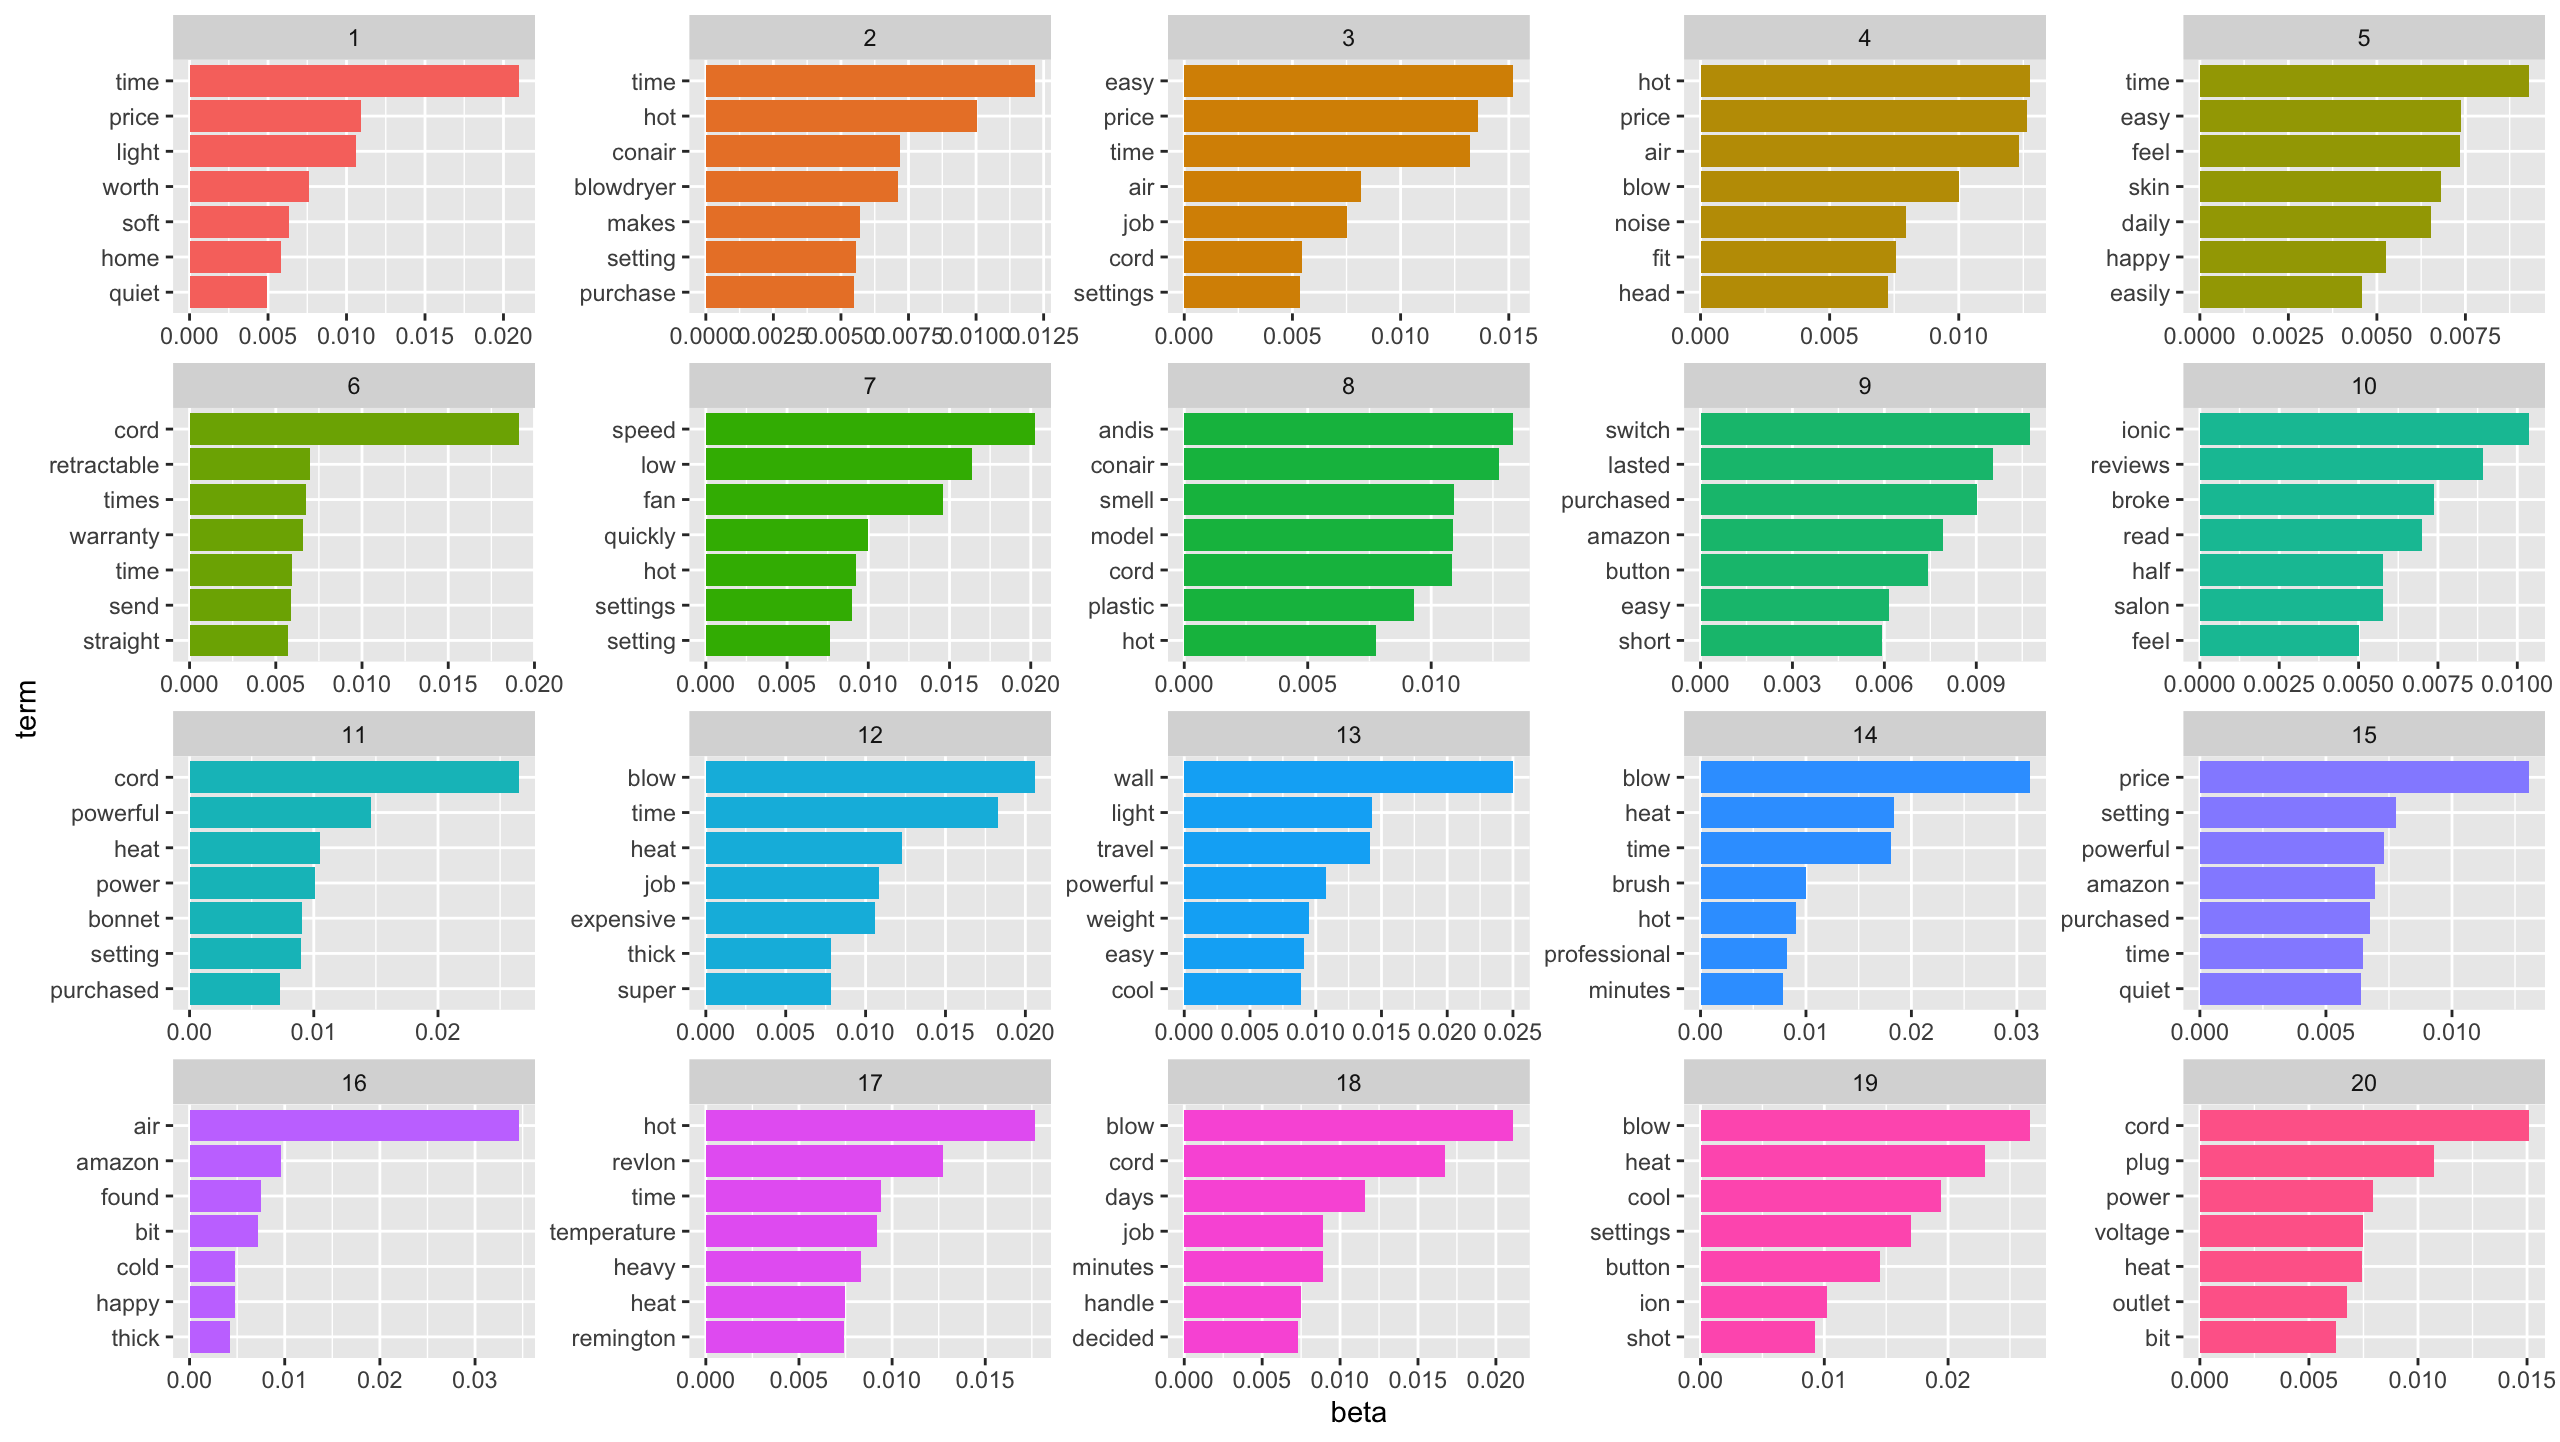
\includegraphics[width= \linewidth]{hair_dryer_top_terms.png}
    \label{fig:sfig1}
    \caption{Hair dryer}
\end{center}
\end{subfigure}
\begin{subfigure}{\textwidth}
\begin{center}
    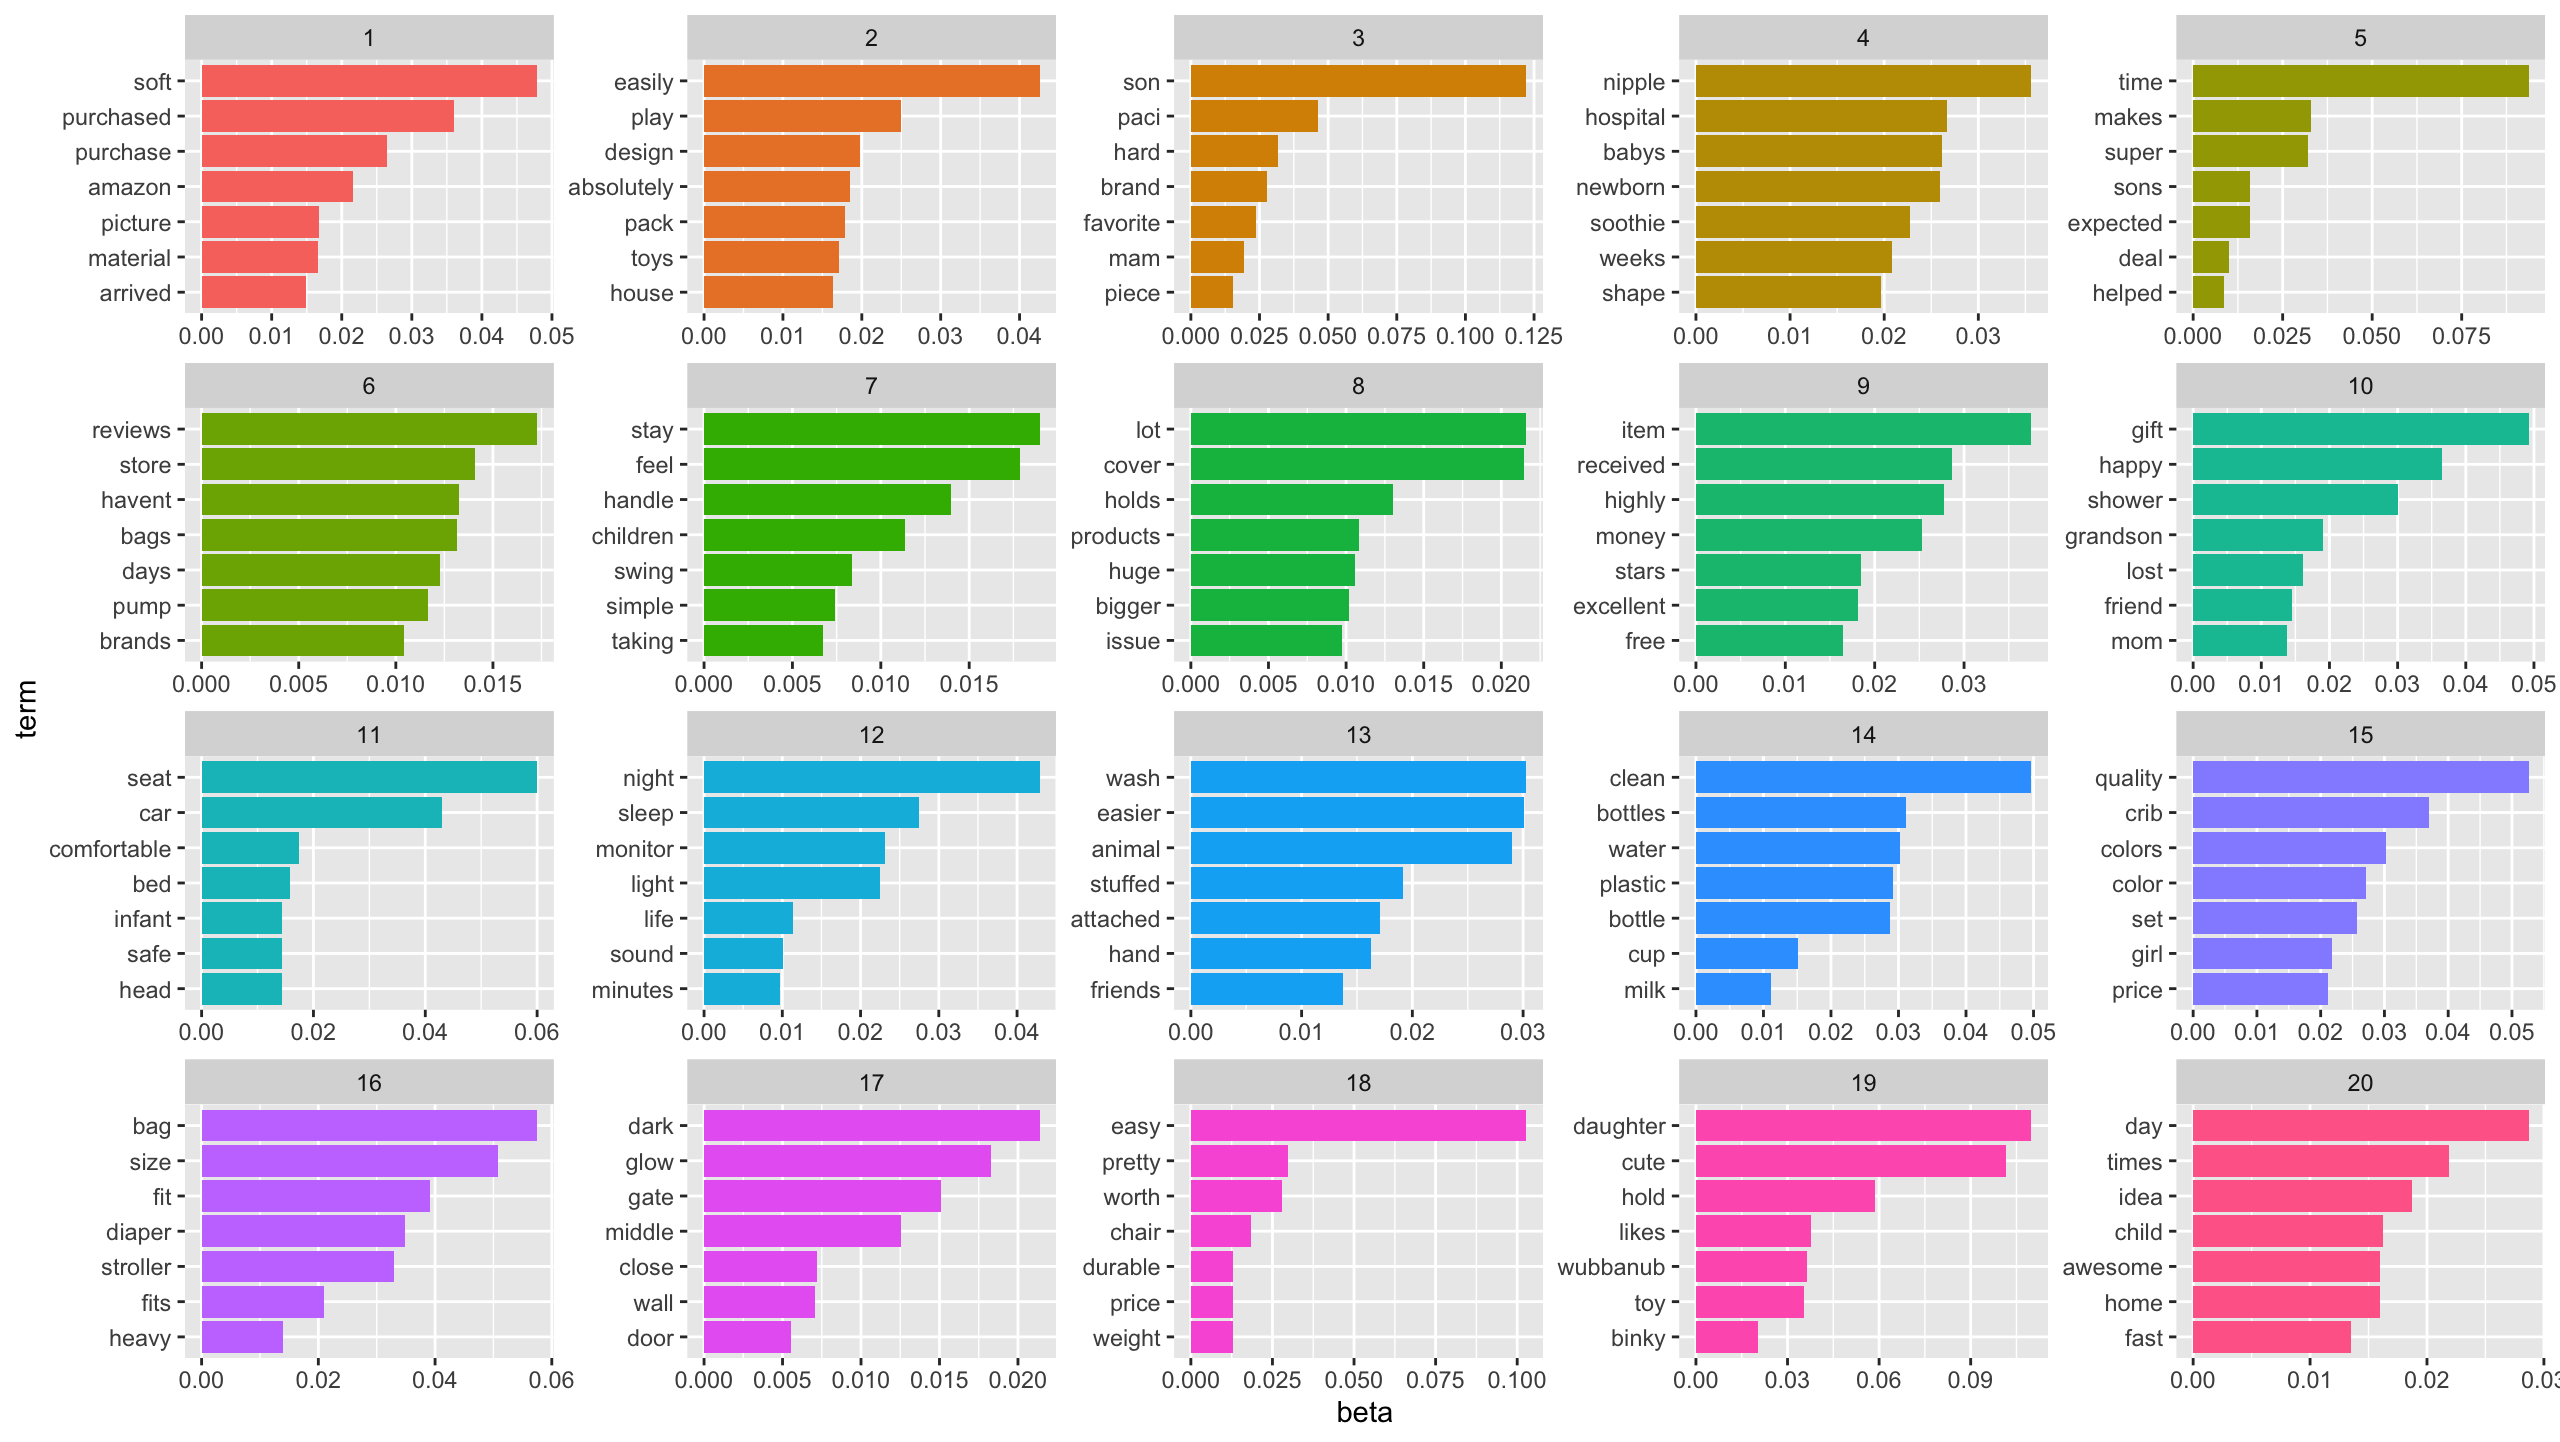
\includegraphics[width= \linewidth]{pacifier_top_terms.png}
    \label{fig:sfig2}
    \caption{Pacifier}
\end{center}
\end{subfigure}
\end{figure}
\begin{figure}{\textwidth}
\begin{center}
    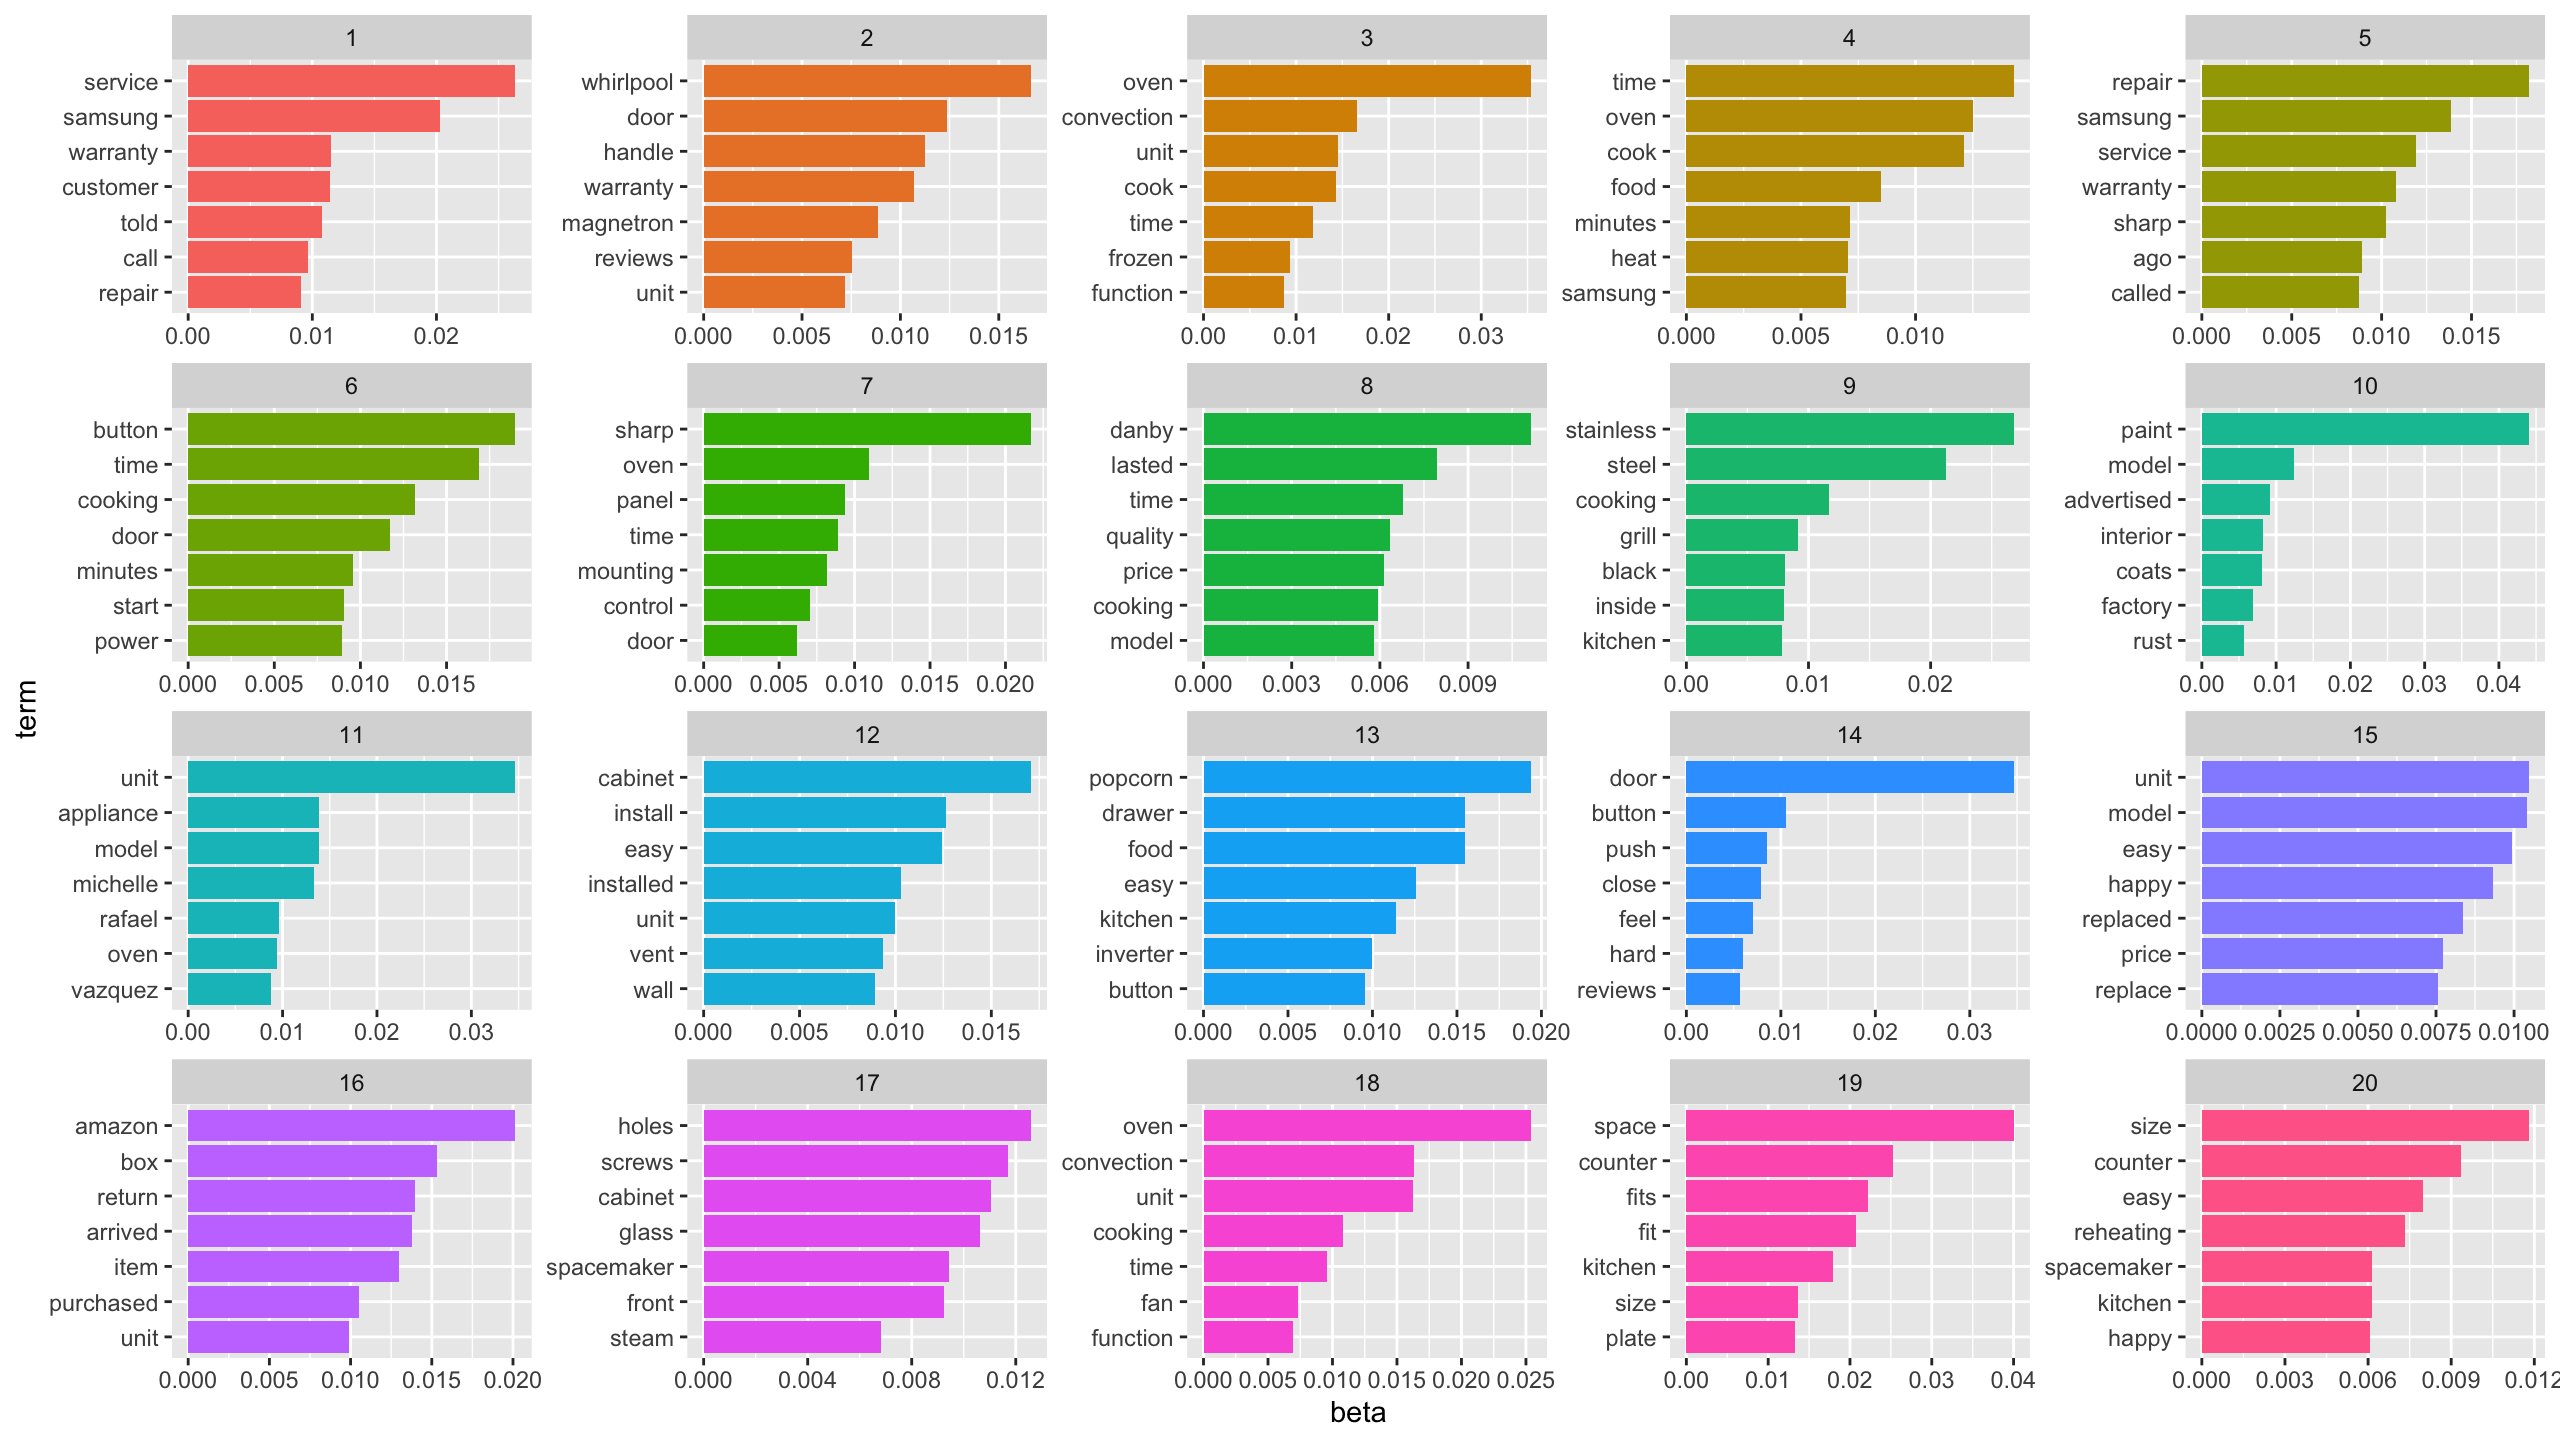
\includegraphics[width= \linewidth]{microwave_top_terms.png}
    c) Microwave
    \end{center}
\end{figure}
\clearpage
\subsection{Product success prediction with binary logistic regression algorithm}
There are two aspects of product success: expected sales, which is based on whether verified purchase is made, and customer satisfaction based on the polarity of reviews. \\
Logistic regression is a supervised learning classification algorithm, which we use to find conditional probability of verified purchase, which ranges from 0 to 1, given one or a combination of feedback indicators. 
Let this probability be $P(y=1|x;w) = p(X)$, where $X = $ a verified purchase is made and $X \sim B(1, p)$.
\subsubsection{Model design}
This model is based on a standard logistic Sigmoid function, defined by $y = \frac{1}{1+e^{-x}}$. Let $\vec{x} = \{x_1, x_2, ..., x_n\}$ be our feature vector of $n$ independent variables. Similarly to linear regression model, our response variable, which is verified purchase, can be expressed as a a linear combination of a weight vector $\vec{w} = \{w_1, w_2, ..., w_n\}$ and the feature vector, plus a bias term $w_0$: $$w_0 + w_1x_1 + w_2x_2+...+w_nx_n = w^{T} \cdot \vec{x}$$
Substituting into the logistic function, we have: $$p(X) = \frac{1}{1+e^{-\vec{w}^{T} \cdot \vect{x}}}$$ 
From the Sigmoid function, $p(X)(1+e^{-\vec{w}^{T} \cdot \vec{x}}) = 1 \implies  \frac{1}{e^{-\vec{w}^{T} \cdot \vect{x}}} = \frac{p(X)}{1-p(X)}$. Thus, the log-odds ratio, which is the log ratio of whether a purchase is likely to occur to whether a purchase is not likely to, is defined by: $$\ln \frac{p(X)}{1-p(X)}=\vec{w}^{T} \cdot \vec{x}$$
We must estimate the parameter vector such that the likelihood function $L(\vec{w}|y) = \Pi_{i=1}^n P(y=1|x;w)^{y_i}_{i} (1-P(y=1|x;w))^{1-y_i}_i$ is maximized. Taking the natural logarithm of the function, we have the log-likelihood function defined as: $$\ell(\vec{w}|y) = \ln (\sum_{i=1}^n P(y=1|x;w)^{y_i}_i + \sum_{i=1}^n(1-P(y=1|x;w))^{1-y_i}_i)$$
The cost function, which is the negative log-likelihood, is to be minimized by a method called gradient descent. We take the partial derivative with respect to each $w_n$ term of the weight factor to eventually get:
$$\frac{\partial \ell(w)}{\partial w} = \sum_{i=1}^{n}(y - P(y=1|x,w))\vec{x}^T$$\\
The gradient descent is then defined as: $$w_{i,j} := w_{i,j}-\alpha(\frac{\partial \ell(w)}{\partial w})$$
\subsubsection{Implementation and results}
We fixed our dependent variable to be verified purchase, which is either $0$ or $1$, and varied our set of independent variables among star ratings, helpful votes, year, average review sentiment, assuming these variables do not have very strong correlation with each other. \\
We denote the following:
\begin{itemize}
    \item $y$: probability of verified purchase, ranging from 0 to 1
    \item $x_1$: log scale of helpful votes
    \item $x_2$: star rating
    \item $x_3$: year
    \item $x_4$: exponential scale of average sentiment of review
\end{itemize}
We look at the magnitude of z-value and estimated coefficient to infer the significance of each feature in predicting verified purchase. Hence,
for pacifier and hair dryer, the most important feature is year, while it is star rating for microwave. The second most important feature is $x_1$, $x_4$ and $x_2$ for pacifier, microwave and hair dryer respectively.
\clearpage
\begin{center}
Table A. Logistic regression model on prediction of sales of 3 products
\begin{table}[]
    \centering
    \begin{tabular}{|c|c|c|c|c|}
    \hline
    \multicolumn{5}{|c|}{Pacifier}\\
    \hline
    Variables & Estimated coefficients &  Standard Error & z-value & p-value \\
    \hline
    Intercept  & -0.18270 &   0.07854  &-2.326 &  0.0200 \\
    $x_1$ & -0.18270 &   0.07854  &-2.326  & 0.0200   \\
    $x_2$ & 0.06205  &  0.04731  & 1.312  & 0.1896 \\
    $x_3$ & 0.34024 &   0.02363 & 14.401   & $<2e^{-16}$ \\
    $x_4$ & 0.55304  &  0.23712  & 2.332 & 0.0197 \\
    \hline
    \end{tabular}
    \begin{tabular}{|c|c|c|c|c|}
    \hline
    \multicolumn{5}{|c|}{Microwave}\\
    \hline
    Variables & Estimated coefficients &  Standard Error & z-value & p-value \\
    \hline
    Intercept  &  -4.76166  &  1.09822 & -4.336& $1.45e^{-5}$ \\
    $x_1$ & -0.22997   & 0.16528  &-1.391  & 0.1641\\
    $x_2$ & 0.79494  &  0.09383  & 8.472 & $<2e^{-16}$ \\
    $x_3$ &0.13326  &  0.07394  & 1.802  & 0.0715 \\
    $x_4$ &1.30509  &  0.69129 &  1.888 &  0.0590 \\
    \hline
    \end{tabular}
    \begin{tabular}{|c|c|c|c|c|}
    \hline
    \multicolumn{5}{|c|}{Hair dryer}\\
    \hline
    Variables & Estimated coefficients &  Standard Error & z-value & p-value \\
    \hline
    Intercept  & -2.66928 &   0.36250 & -7.364& $1.79e^{-13}$ \\
    $x_1$ & -0.08111 &   0.06827&  -1.188   & 0.235\\
    $x_2$ & 0.20460  &  0.04594  & 4.454 &$8.43e^{-6}$\\
    $x_3$ & 0.33513   & 0.02369 & 14.146 & $< 2e^{-16}$ \\
    $x_4$ & 0.02487  &  0.24038  & 0.103 &   0.918     \\
    \hline
    \end{tabular}
\end{table}
\end{center}
\subsection{Predict future customer behavior in response to star rating}
We first define the following, for a certain product:
\begin{itemize}
    \item $n$: time step
    \item $S_n$: star rating at time step $n$
    \item $R_n$: review count at time step $n$
    \item $Q_n$: review quality at time step $n$, determined by total helpful votes of all reviews
    \item $T_n$: review sentiment at time step $n$
\end{itemize}
If we hypothesize that future customer behavior, including future review quantity, quality and sentiment, would be immediately influenced by current star rating, we can formalize a multi-variable, deterministic discrete linear model as follows:
\begin{align*}
S_{n+1} & = \, a_1 \cdot S_n + b_1 \cdot R_n + c_1 \cdot Q_n + d_1 \cdot T_n+ e_1 \\
R_{n+1} & = \, a_2 \cdot S_n + b_2 \cdot R_n + c_2 \cdot Q_n + d_2 \cdot T_n + e_2 \\
Q_{n+1} & = \, a_3 \cdot S_n + b_3 \cdot R_n + c_3 \cdot Q_n + d_3 \cdot T_n+ e_3 \\
T_{n+1} & = \, a_4 \cdot S_n + b_4 \cdot R_n + c_4 \cdot Q_n + d_4 \cdot T_n+ e_4 \\
\end{align*}
We treat our system of linear equations as a system that evolves over time, thus we can use the diagonalization to describe such a system. We use this method to identify how our variables change over time. \\
Assuming the constant terms $e_1, e_2, e_3, e_4$ are all 0, our system is first-order homogeneous linear equation. Let us treat our system of linear equations as the matrix A, where A=
$$
\begin{bmatrix}
a_1&b_1&c_1&d_1\\
a_2&b_2&c_2&d_2\\
a_3&b_3&c_3&d_3\\
a_4&b_4&c_4&d_4\\
\end{bmatrix}
$$
then by diagonalization, \(A=P\cdot D\cdot P^{-1}\). Therefore we can write $A^k=P\cdot D^k\cdot p^{-1}$, where k represents time. By theorem we know that A is diagonalizable if and only if has eigenvectors \textbf{\(x_1,x_2,....x_n\)}such that the matrix $P=[x_1 x_2 ... x_n]$ is invertible and since P is invertible then we have $P^{-1}$. When this happens $P^{-1}\cdot A\cdot P= diag(\lambda_1,\lambda_2,\cdots, \lambda_n)$, where for each i, $\lambda_i$ is the eigenvalue of A corresponding to $x_i$ the eigenvectors. Our matrix D will inform us on how our system will evolve. It is more likely that if a variable is associated with a $\lambda_i>1$ then that variable will grow.
\section{Letter to Sunshine company}
Dear Sunshine Company,\\
We write this letter to inform you on important data measures and important design features you need to know to enhance your products. We use linear and logistic regression models to identify important data measures. To predict future sales, you may want to look at review sentiments, number of helpful votes for reviews and may not consider looking at star rating as star rating does not seem to impact the prediction models much. We identify the important features based on frequency of words over all reviews. The most common features across all products that customers focus on is ease of use. Specifically, pacifier's features include durability, material and appearance. Microwave's features include material and occupied space. Hair dryer's important features include heating element and weight. \\
We hope this helps in informing you to make sound marketing decisions. Thank you for your time. \\
Yours sincerely,\\
Team 2022849
\section{Appendix}
\subsection{Softwares and packages}
We processed our data and built our prediction models with the help of Excel and the following Python and R packages:
\begin{center}
\begin{tabular}{|p{2cm}|p{5cm}|p{8cm}|} 
 \hline
Packages & Functions & Documentation \\
 \hline
 pandas & data analysis and manipulation & \texttt{http://github.com/pandas-dev/pandas} \\
 \hline
 numpy &complex mathematical functions &  \texttt{https://numpy.org/}\\
 \hline
tm  & text processing, create corpus over all reviews  & \texttt{https://cran.r-project.org/ web/packages/tm/tm.pdf}\\
\hline
dplyr & manipulation of data sets & \texttt{https://cran.r-project.org/ web/packages/dplyr/dplyr.pdf}\\
 \hline
tidytext  &  text mining for word processing and sentiment analysis& \texttt{https://cran.r-project.org/ web/packages/tidytext/tidytext.pdf}\\
\hline
qdap & text processing & \texttt{https://cran.r-project.org/web/ packages/qdap/qdap.pdf}\\
\hline
sentimentr  & sentiment analysis of reviews  &
\texttt{http://github.com/trinker/ sentimentr}\\
\hline
ggplot2 & visualization of prediction models & \texttt {https://cran.r-project.org/ web/packages/ggplot2/ggplot2.pdf}\\
\hline
tidyverse  & a set of packages that work in harmony  & \texttt{https://cran.r-project.org/ web/packages/tidyverse/tidyverse.pdf}\\
\hline
topicmodels & create document-terms-matrix, build LDA models  & \texttt{https://cran.r-project.org /web/packages/topicmodels/topicmodels.pdf}\\
\hline
broom & summarizing key information in the form of tidy tibbles for faster reporting & \texttt{https://cran.r-project.org/ web/packages/broom/broom.pdf}\\
 \hline
\end{tabular}
\end{center}
\subsection{Figures}
\begin{figure}[htbp]
\caption{Lines and residuals plots for 3 products:}
\begin{subfigure}{\textwidth}
    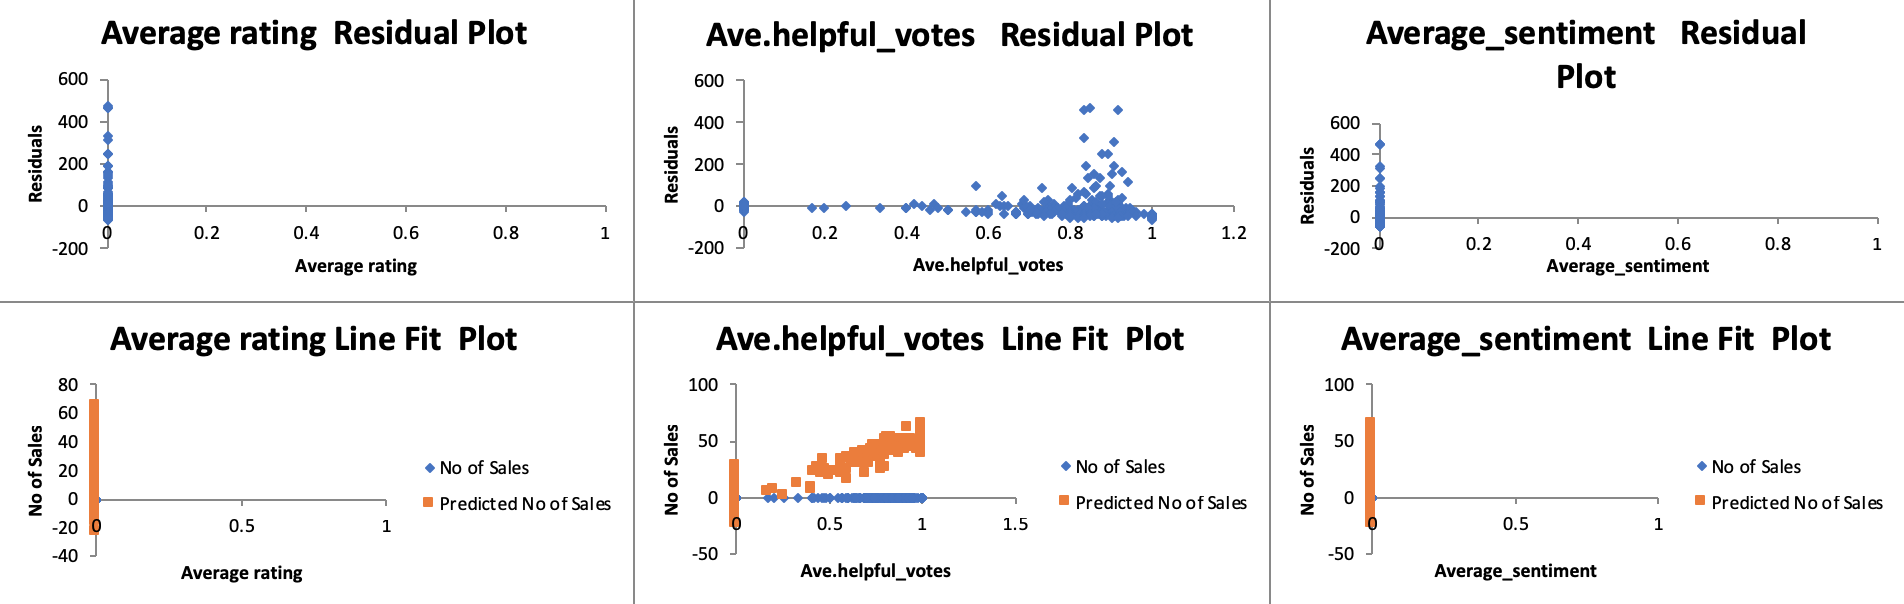
\includegraphics[width= 1\linewidth]{hair_dryer_lines_residuals}
    \label{fig:sfig1}
    \caption{Hair dryer}
    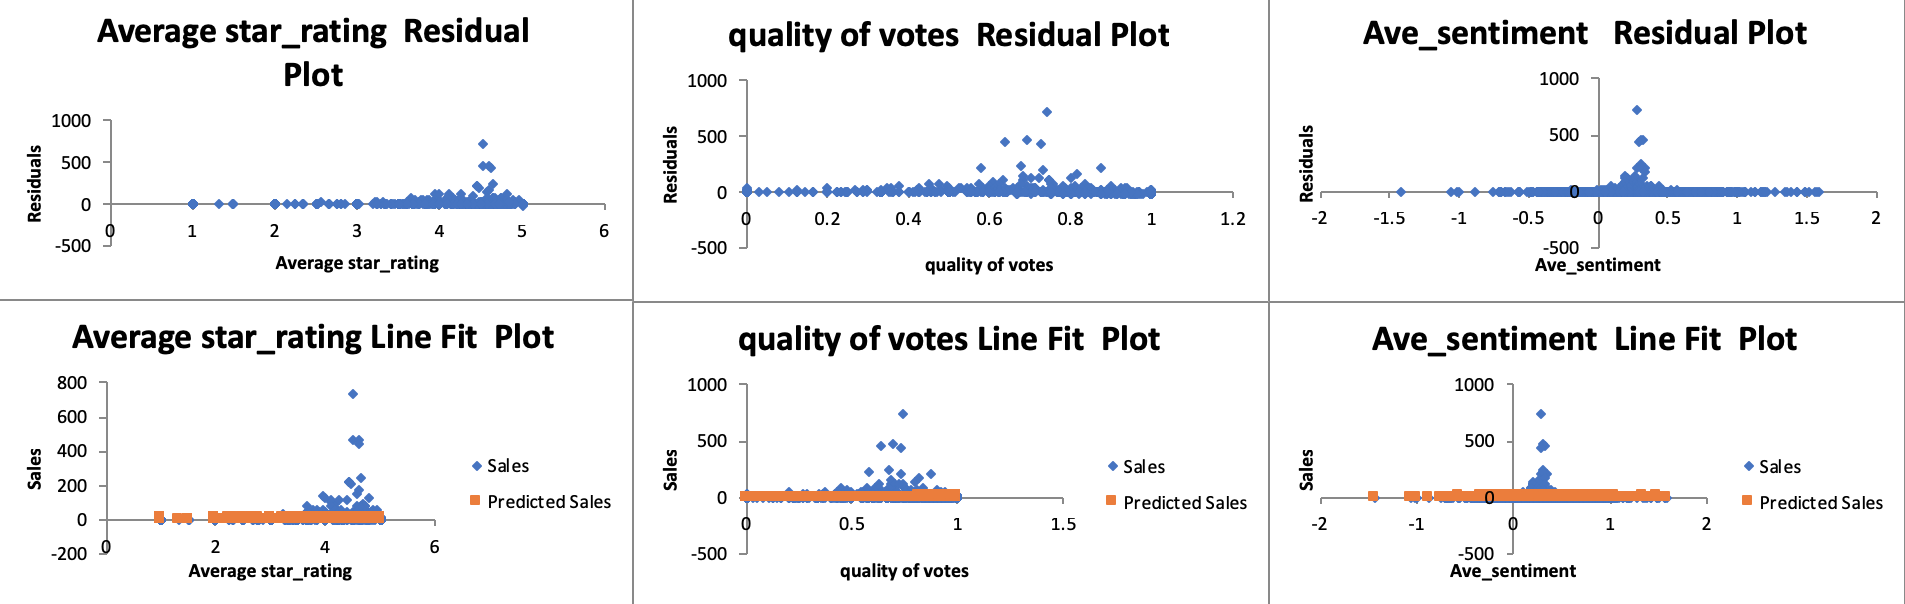
\includegraphics[width= 1\linewidth]{pacifier_lines_residuals}
    \label{fig:sfig2}
    \caption{Pacifier}
    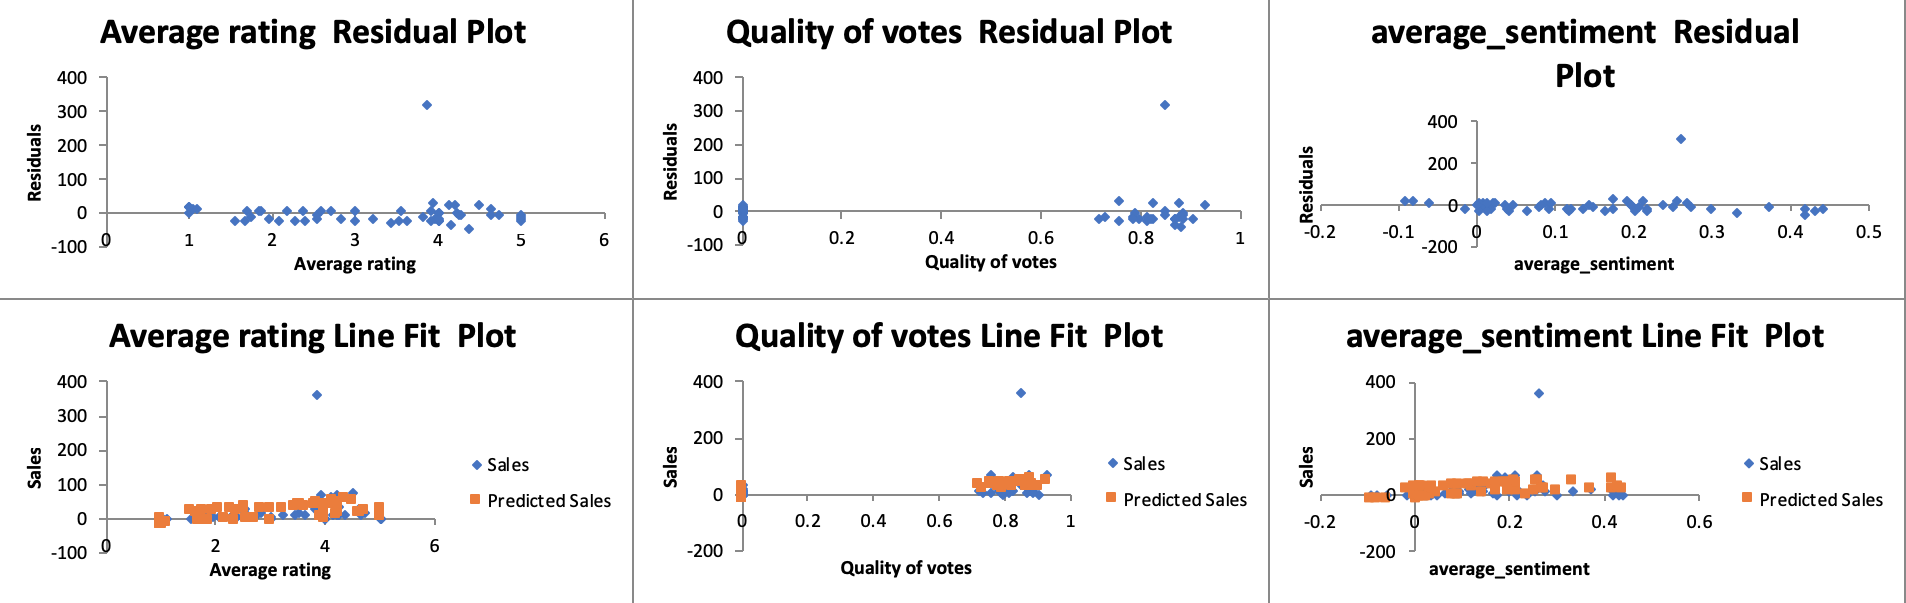
\includegraphics[width= 1\linewidth]{microwave_lines_residuals}
    \label{fig:sfig3}
    \caption{Microwave}
\end{subfigure}%
\end{figure}
\begin{figure}[htbp]
\caption{Perplexity score against k for 3 products:}
\begin{subfigure}{\textwidth}
\begin{center}
    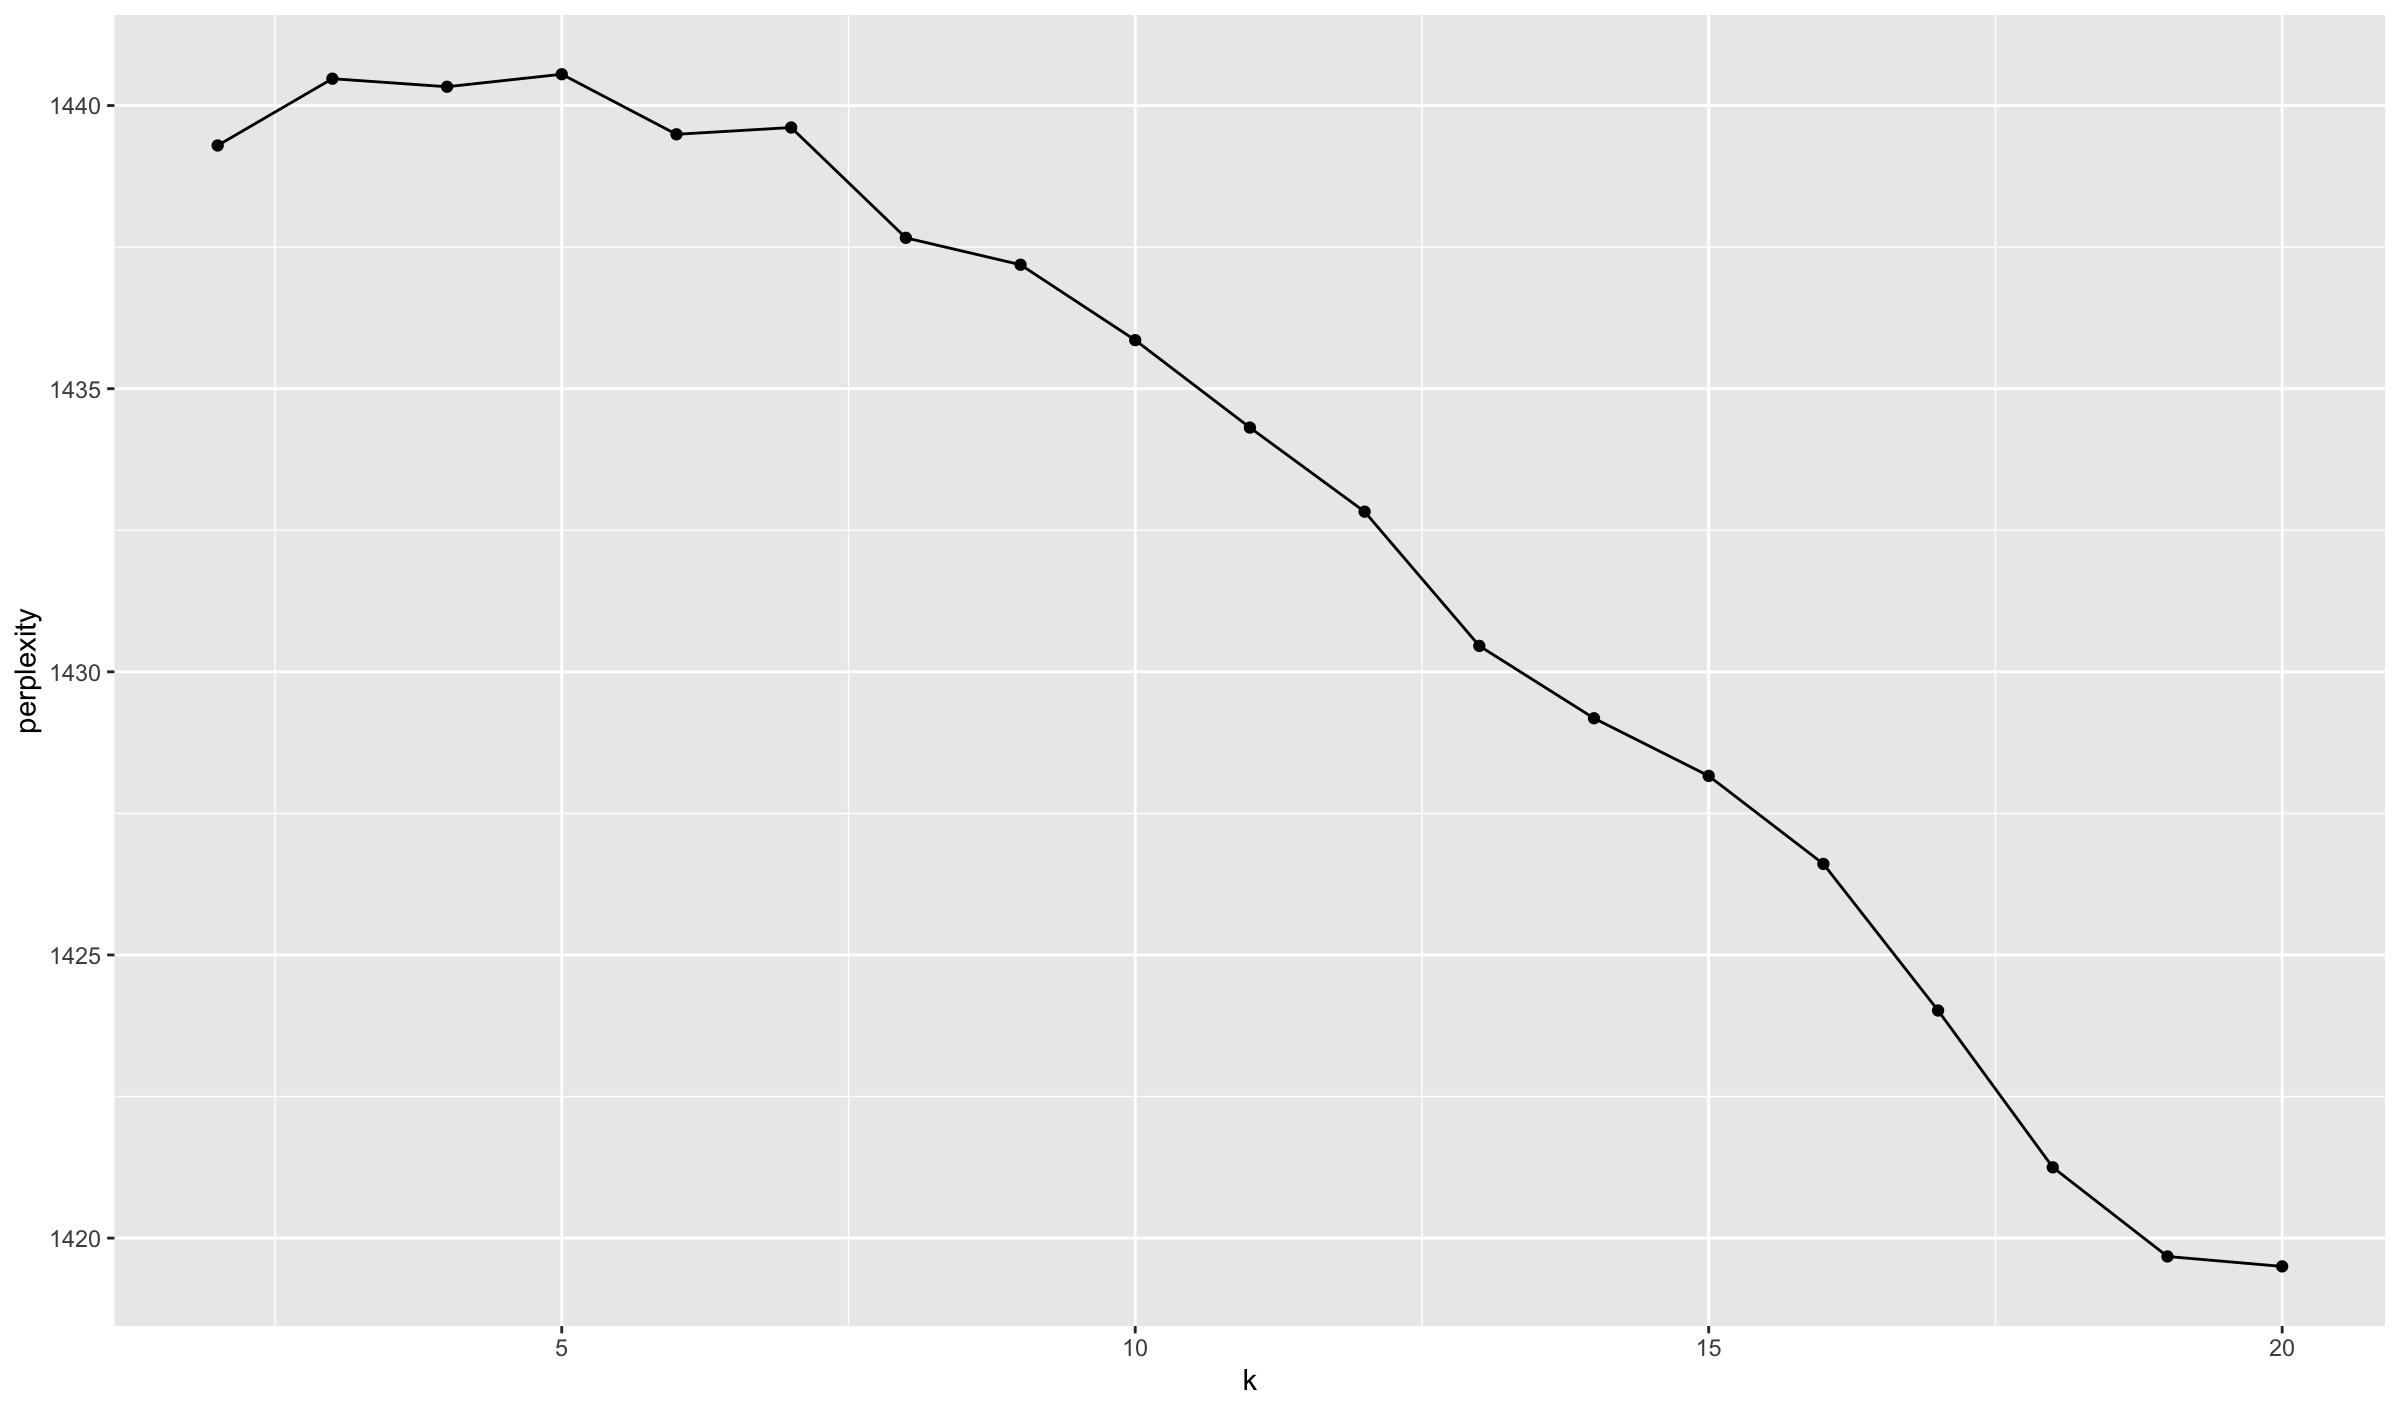
\includegraphics[width= .7\linewidth]{hair_dryer_perplexity.png}
    \label{fig:sfig1}
    \caption{Hair dryer}
\end{center}
\end{subfigure}
\begin{subfigure}{\textwidth}
\begin{center}
    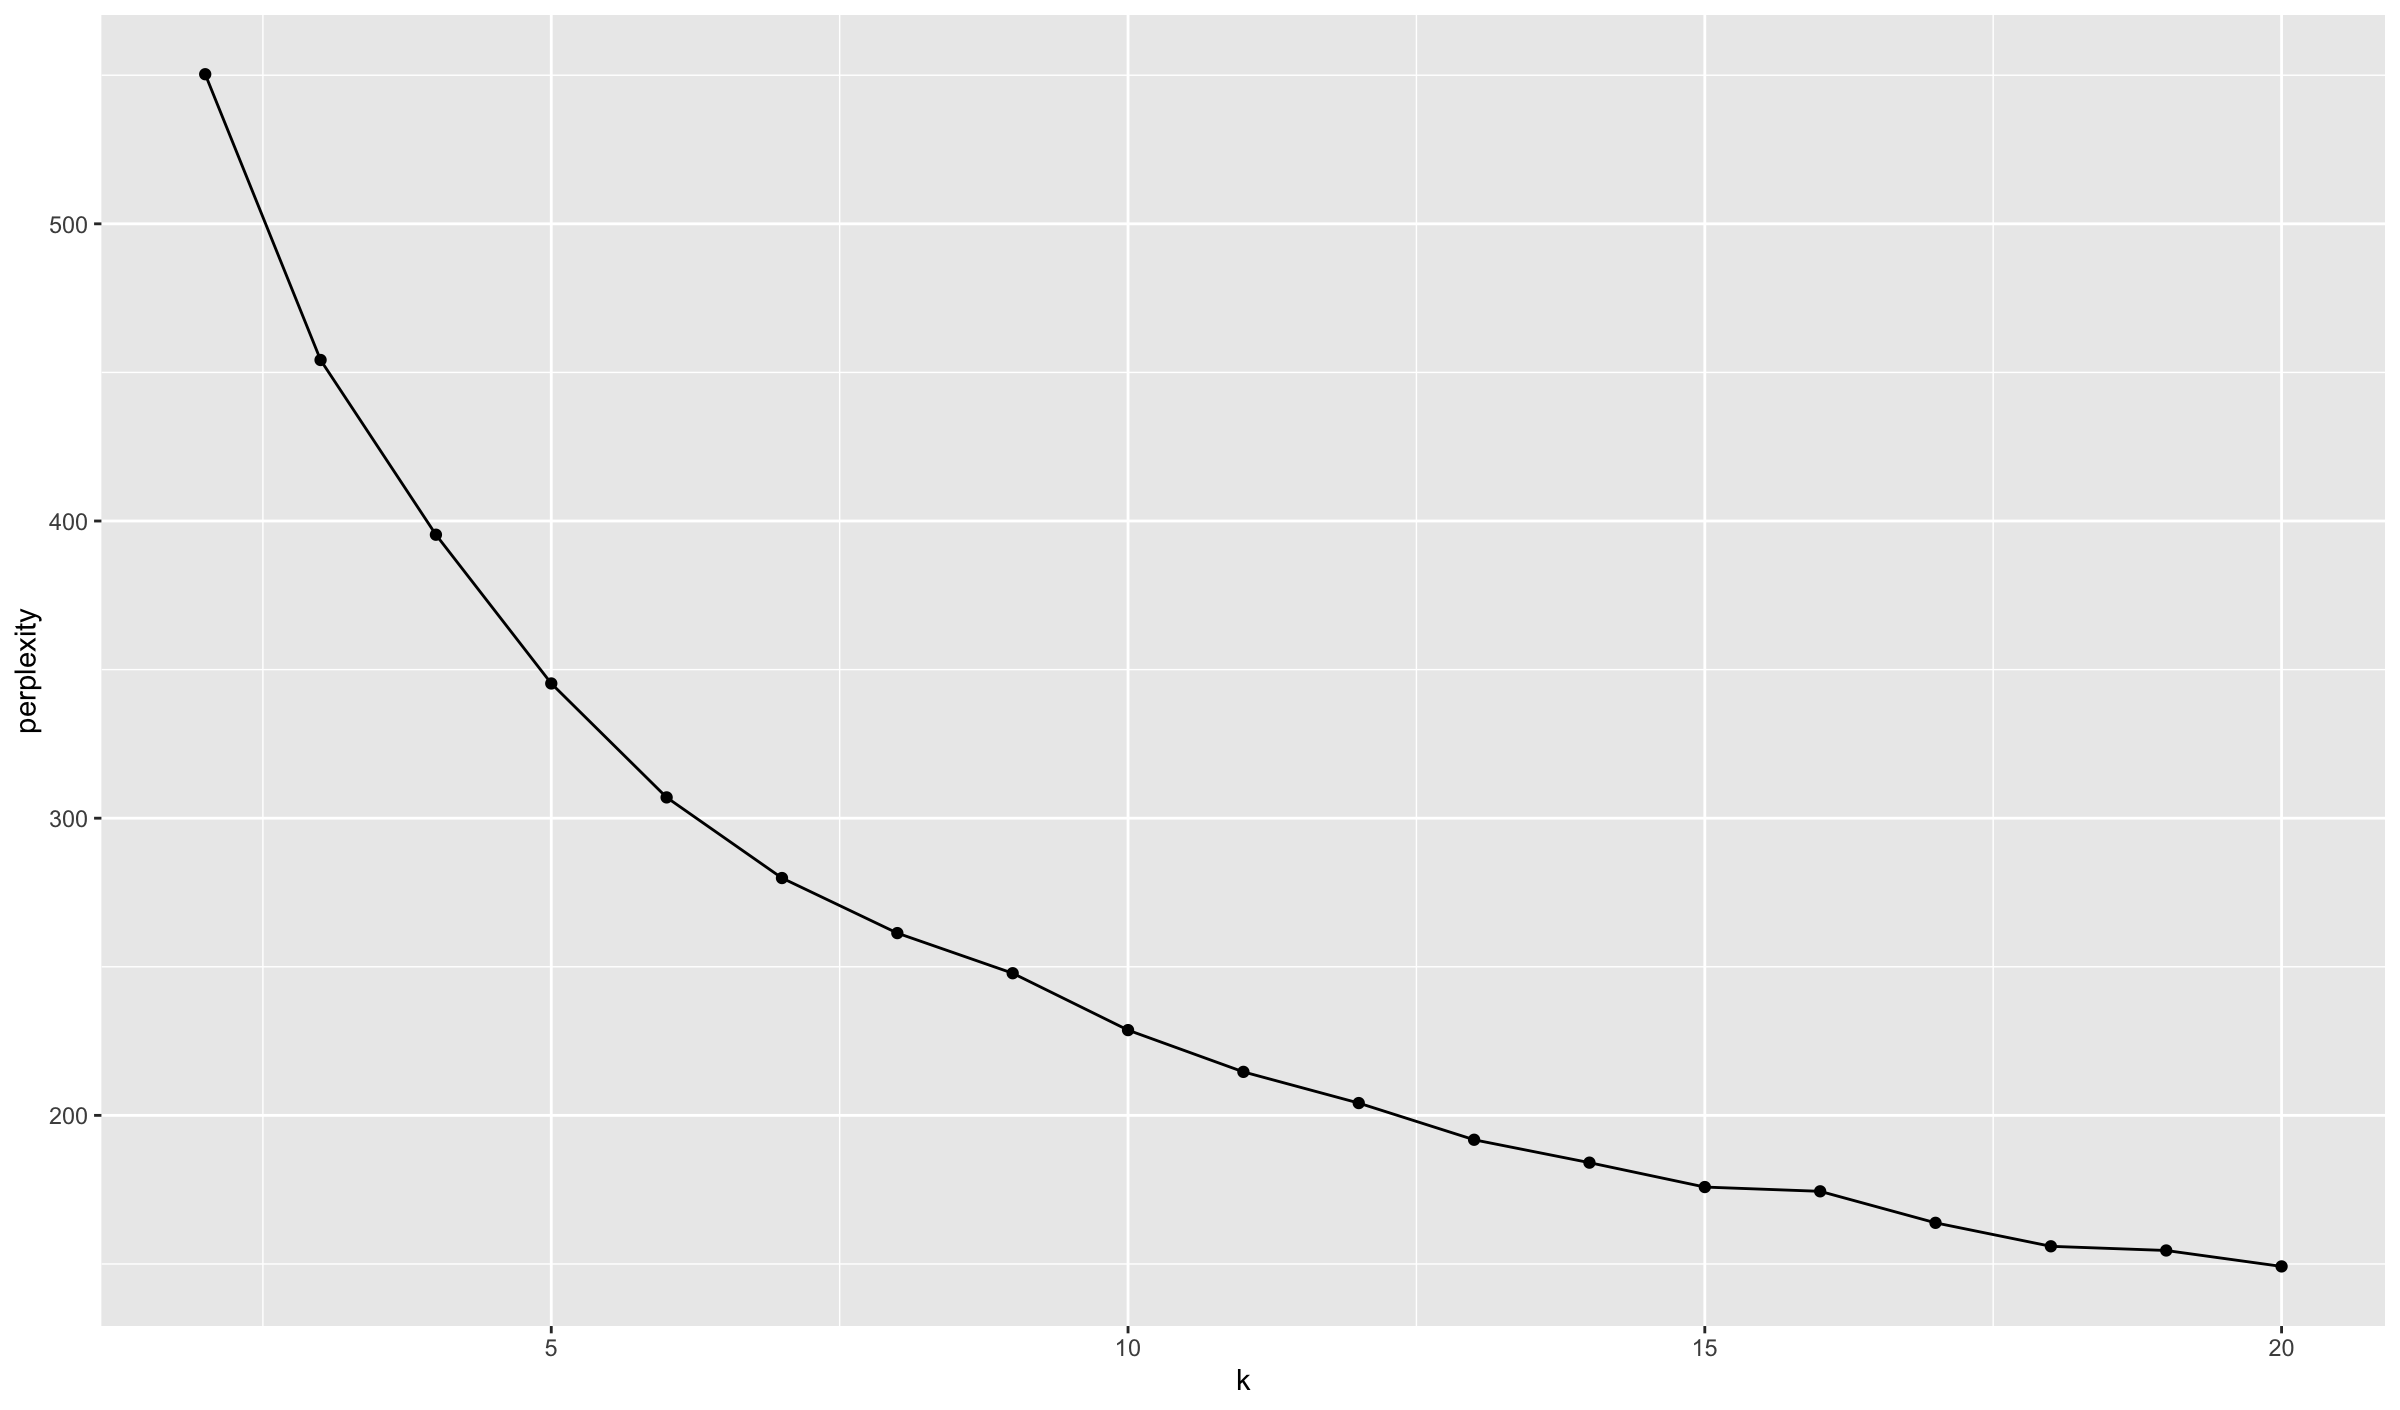
\includegraphics[width= .7\linewidth]{pacifier_perplexity.png}
    \label{fig:sfig2}
    \caption{Pacifier}
\end{center}
\end{subfigure}
\begin{subfigure}{\textwidth}
\begin{center}
    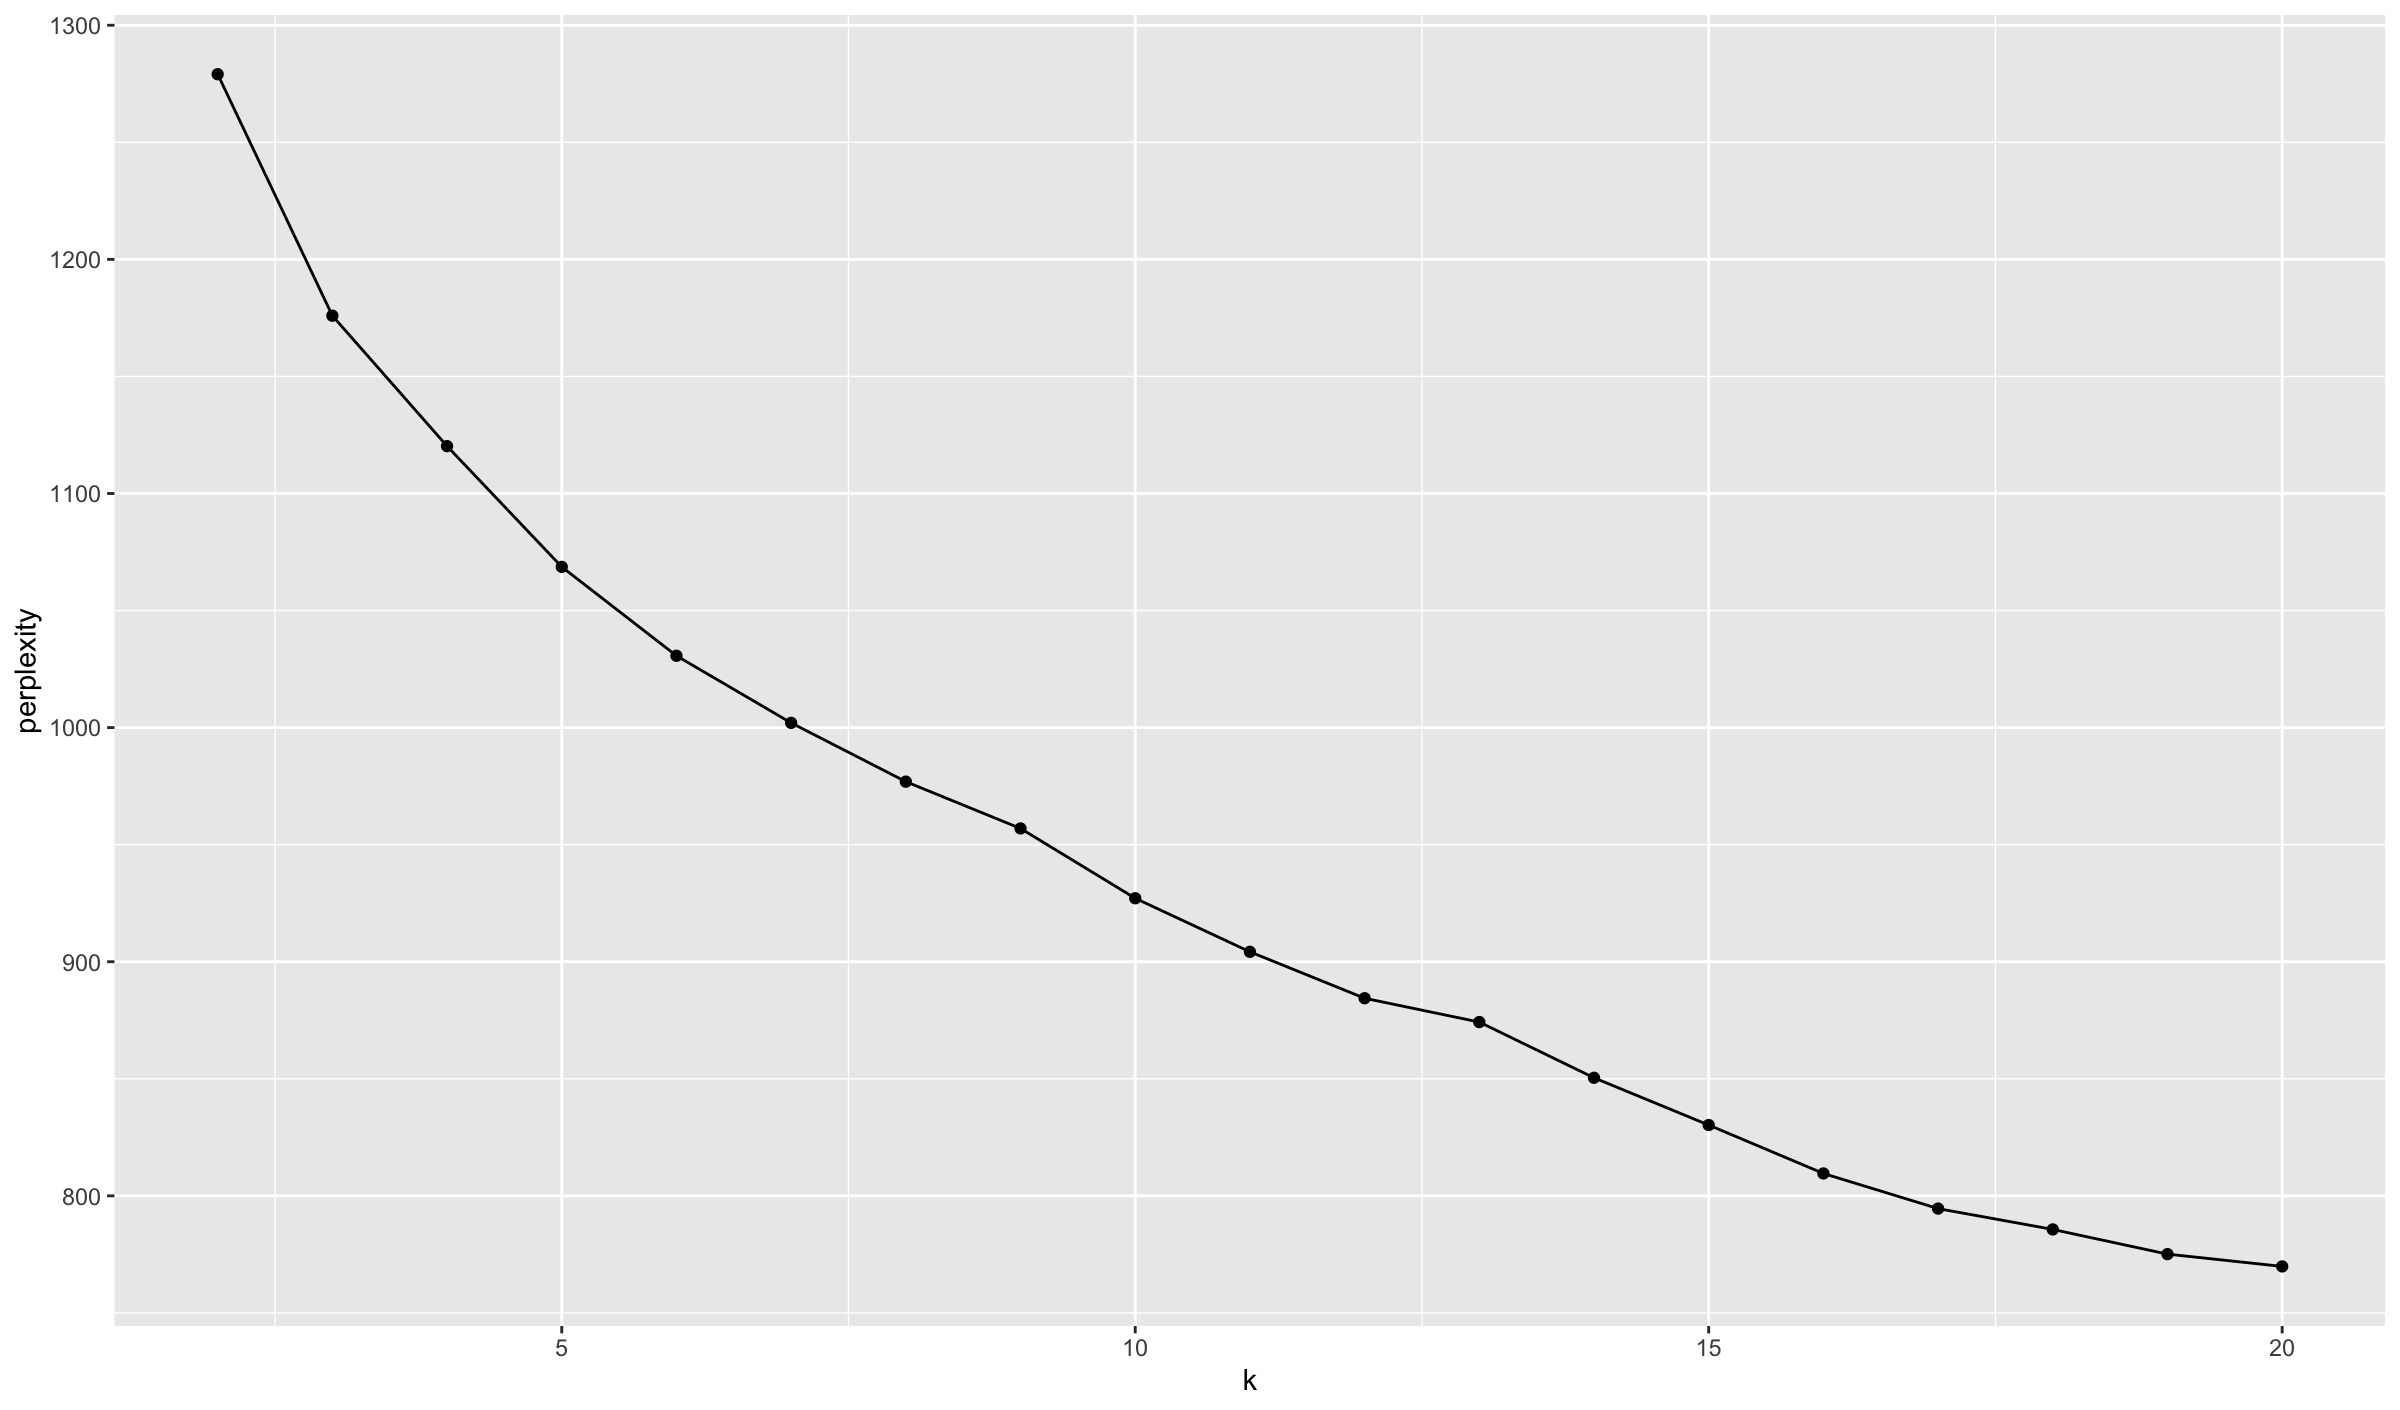
\includegraphics[width= .7\linewidth]{microwave_perplexity.png}
    \label{fig:sfig3}
    \caption{Microwave}
    \end{center}
\end{subfigure}
\end{figure}
\begin{figure}[htbp]
\caption{Logistic regression model for 3 products:}
\begin{subfigure}{\textwidth}
\begin{center}
    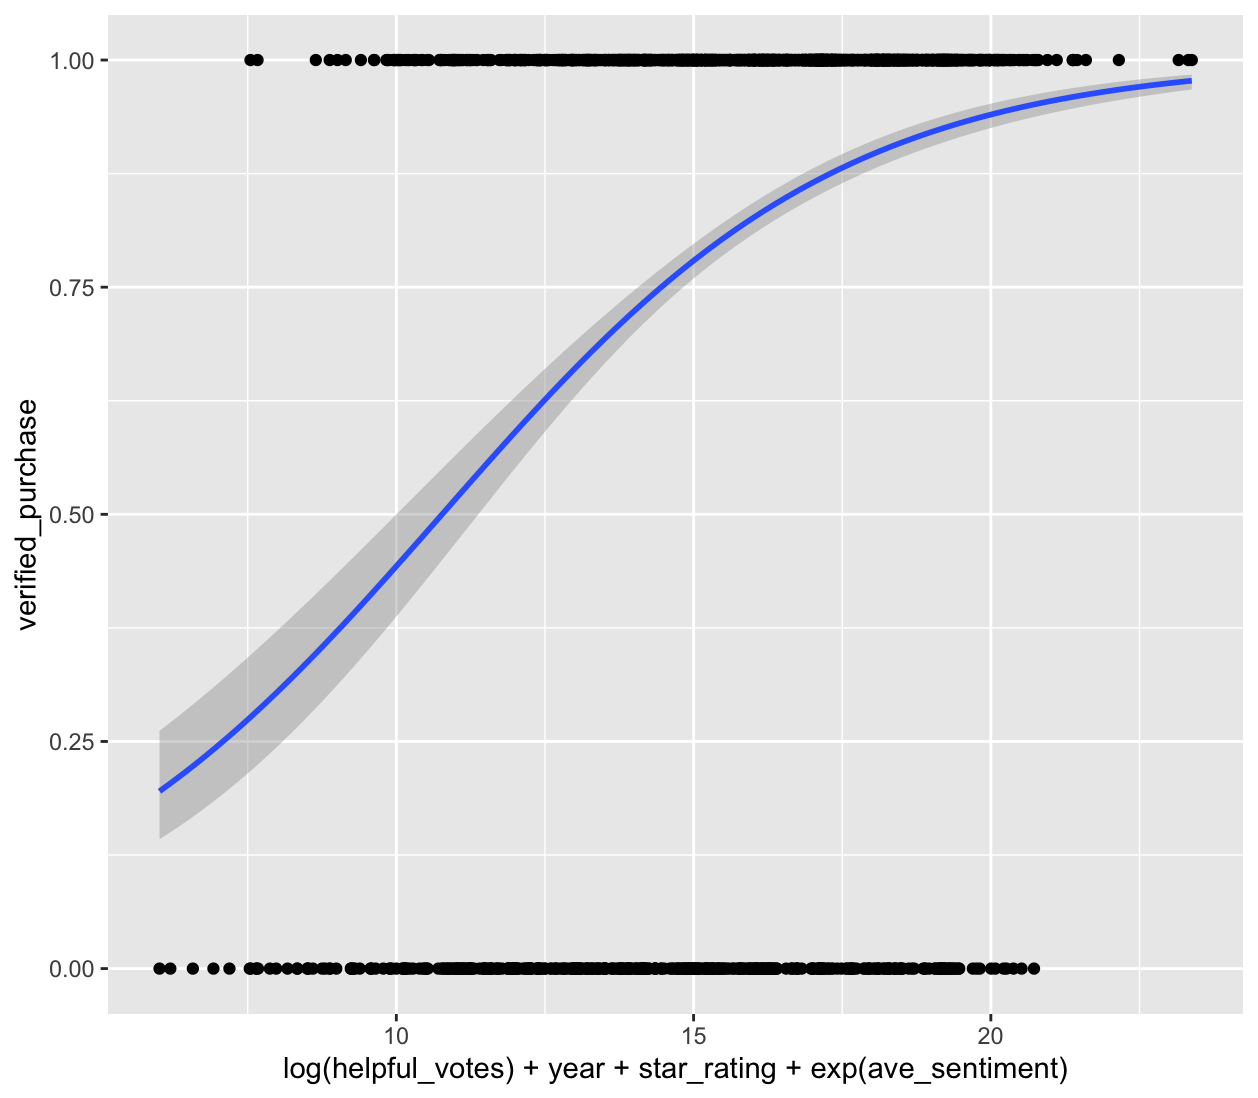
\includegraphics[width= .5\linewidth]{hair_dryer_lg.png}
    \label{fig:sfig1}
    \caption{Hair dryer}
\end{center}
\end{subfigure}
\begin{subfigure}{\textwidth}
\begin{center}
    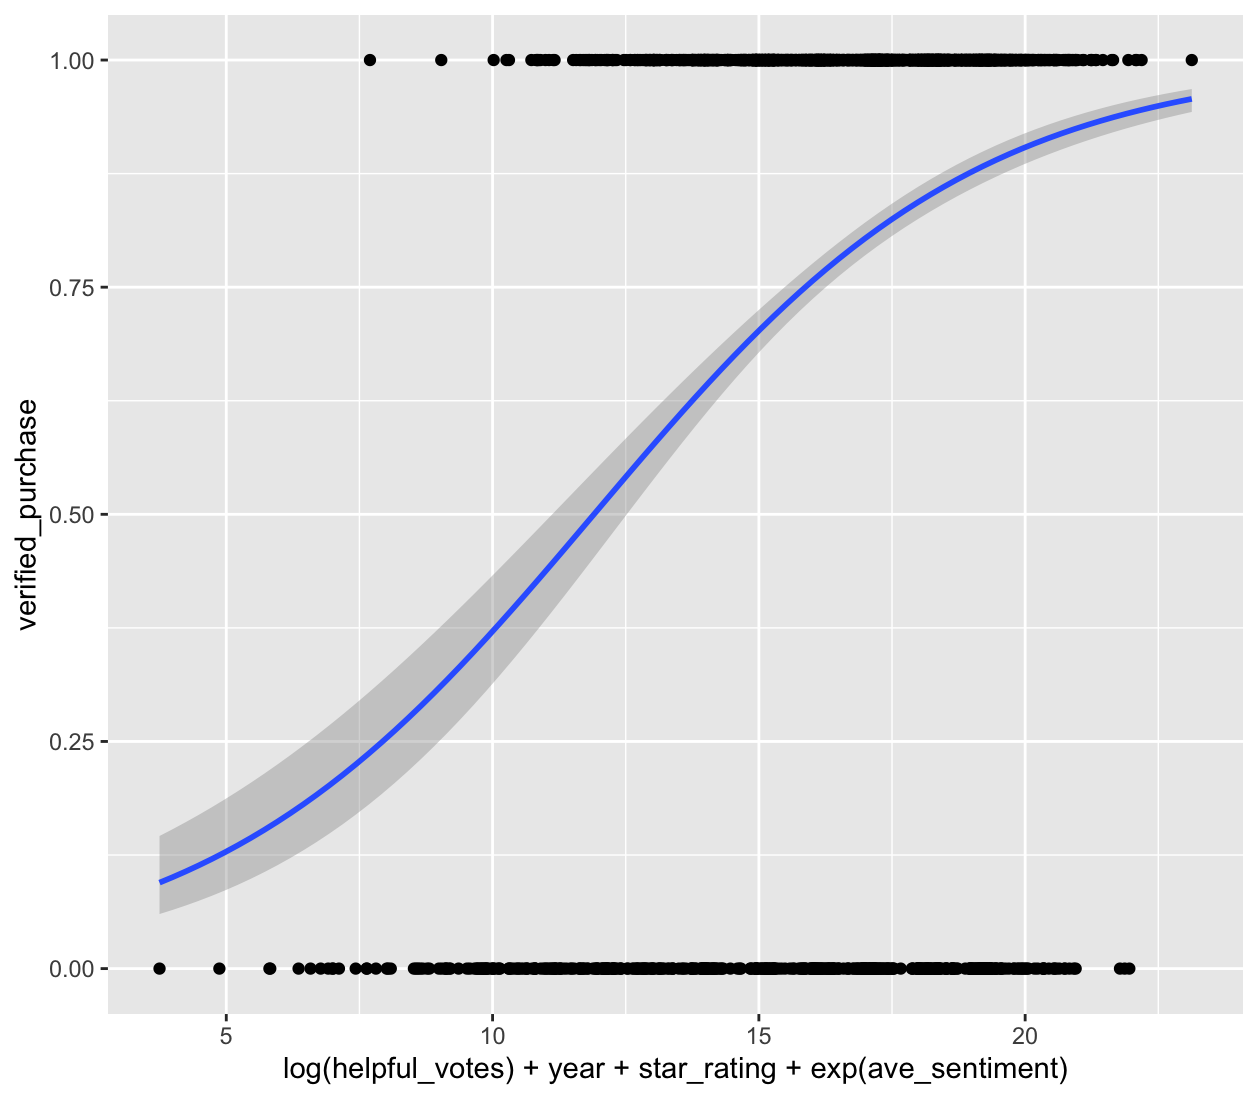
\includegraphics[width= .5\linewidth]{pacifier_lg.png}
    \label{fig:sfig2}
    \caption{Pacifier}
\end{center}
\end{subfigure}
\begin{subfigure}{\textwidth}
\begin{center}
    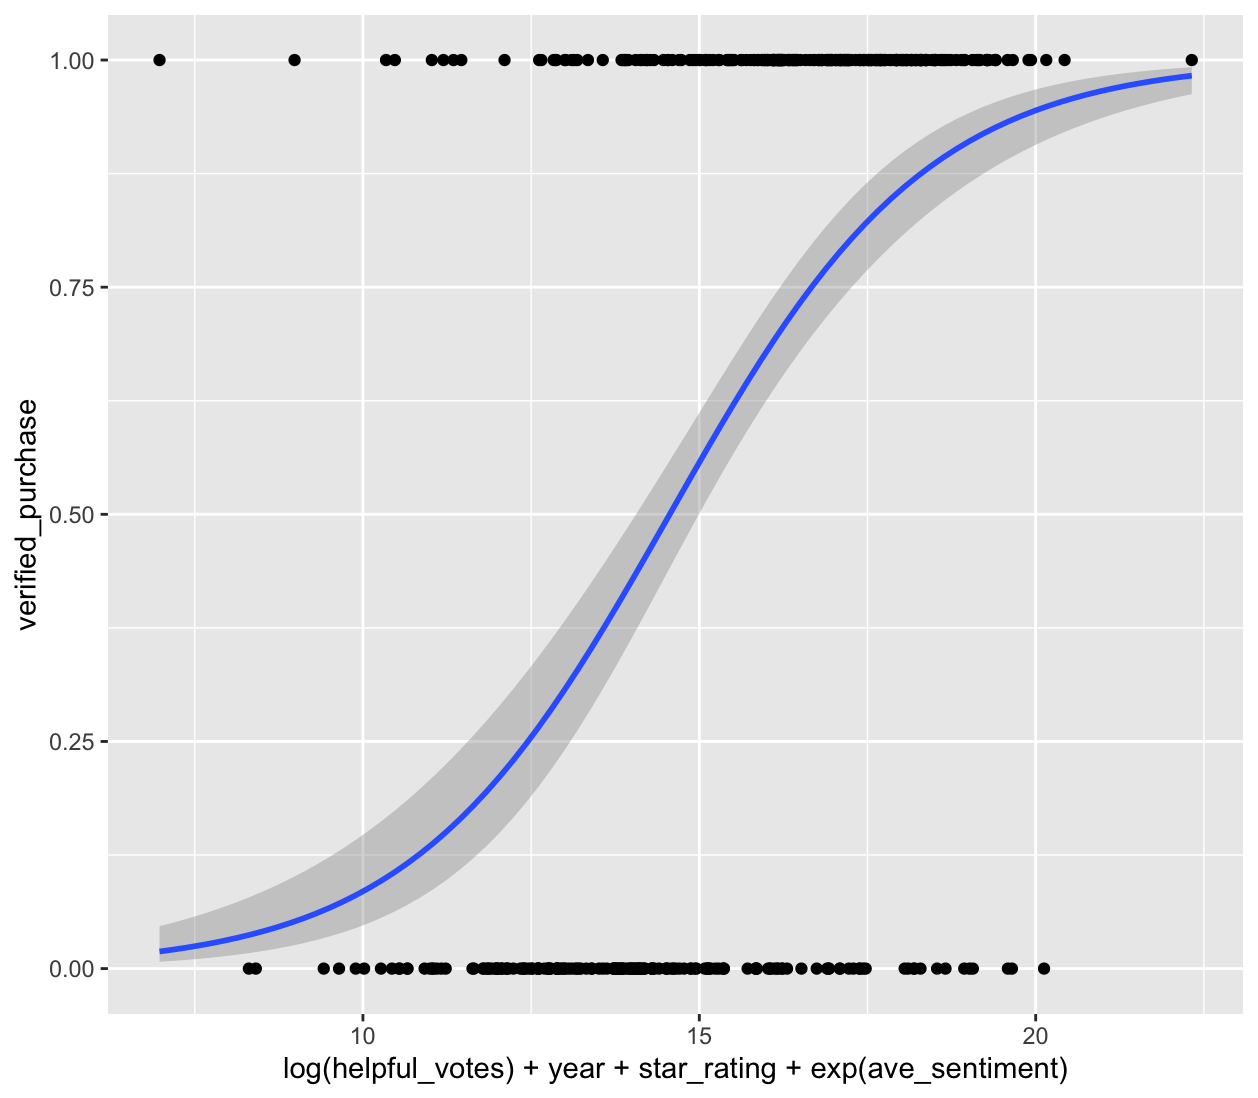
\includegraphics[width= .5\linewidth]{microwave_lg.png}
    \label{fig:sfig3}
    \caption{Microwave}
    \end{center}
\end{subfigure}
\end{figure}
\newpage
\begin{thebibliography}{9}
\bibitem{sentimentr} Rinker, T. W. (2019) \textit{sentimentr: Calculate Text Polarity}, \textit{Sentiment version 2.7.1.} \texttt{http://github.com/trinker/sentimentr}.
\bibitem{Blei_Ng_Jordan} Blei, David M., Andrew Y. Ng, and Michael I. Jordan. \textit{"Latent dirichlet allocation." Journal of machine Learning research}, 3 Jan 2003: 993-1022.
\bibitem{steyvers} Steyvers, Mark, and Tom Griffiths. \textit{"Probabilistic topic models."} \textit{Handbook of latent semantic analysis} 427.7 (2007): 424-440.
\bibitem{2} Fang, Anna, and Zina Ben-Miled. "Does bad news spread faster?." \textit{2017 International Conference on Computing, Networking and Communications (ICNC).} IEEE, 2017.
\end{thebibliography}
\end{document}
